\documentclass[11pt]{article}
\usepackage[textwidth=18.0cm, textheight=23.0cm, top=2.0cm]{geometry}
\usepackage{pst-all}
\usepackage{amssymb}
\usepackage{tikz}
\usepackage{underscore}\begin{document}
\pagestyle{empty}


ClassName: \underline{\textbf{Class_05.2bp-43}}
\par
BinSize: \underline{\textbf{100 × 100}}
\par
ReduceSize: \underline{\textbf{100 × 100}}
\par
TypeNum: \underline{\textbf{100}}
\par
Num: \underline{\textbf{100}}
\par
OutS: \underline{\textbf{260000}}
\par
InS: \underline{\textbf{240023}}
\par
Rate: \underline{\textbf{0.923}}
\par
UB: \underline{\textbf{26}}
\par
LB0: \underline{\textbf{26}}
\par
LB: \underline{\textbf{26}}
\par
LBWithCut: \underline{\textbf{26}}
\par
NodeCut: \underline{\textbf{0}}
\par
ExtendedNodeCnt: \underline{\textbf{1}}
\par
GenNodeCnt: \underline{\textbf{1}}
\par
PrimalNode: \underline{\textbf{0}}
\par
ColumnCount: \underline{\textbf{26}}
\par
TotalCutCount: \underline{\textbf{0}}
\par
RootCutCount: \underline{\textbf{0}}
\par
LPSolverCnt: \underline{\textbf{1}}
\par
PricingSolverCnt: \underline{\textbf{0}}
\par
BranchAndBoundNum: \underline{\textbf{1}}
\par
isOpt: \underline{\textbf{true}}
\par
TimeOnPrimal: \underline{\textbf{0.000 s}}
\par
TimeOnPricing: \underline{\textbf{0.000 s}}
\par
TimeOnRmp: \underline{\textbf{0.078 s}}
\par
TotalTime: \underline{\textbf{0.156 s}}
\par
\newpage


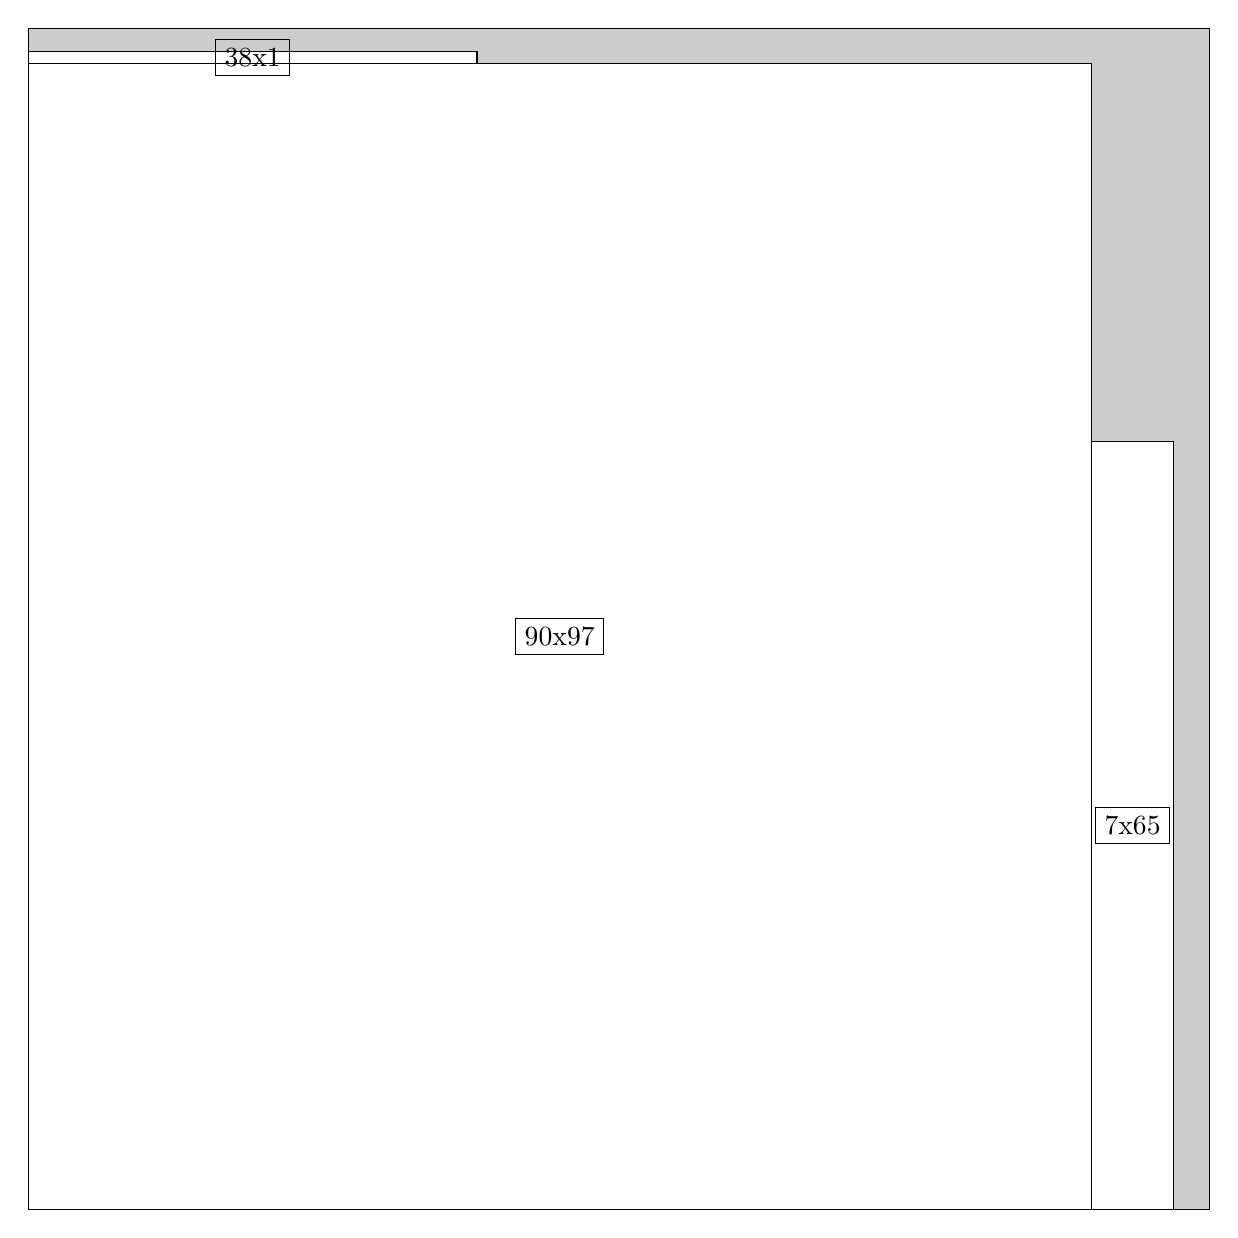
\begin{tikzpicture}[shorten >=1pt,scale=1.0,every node/.style={scale=1.0},->]
\tikzstyle{vertex}=[circle,fill=black!25,minimum size=14pt,inner sep=0pt]
\filldraw[fill=gray!40!white, draw=black] (0,0) rectangle (15.0,15.0);
\foreach \name/\x/\y/\w/\h in {90x97/0.0/0.0/13.5/14.549999999999999,7x65/13.5/0.0/1.05/9.75,38x1/0.0/14.549999999999999/5.7/0.15}
\filldraw[fill=white!40!white, draw=black] (\x,\y) rectangle node[draw] (\name) {\name} ++(\w,\h);
\end{tikzpicture}


w =90 , h =97 , x =0 , y =0 , v =8730
\par
w =7 , h =65 , x =90 , y =0 , v =455
\par
w =38 , h =1 , x =0 , y =97 , v =38
\par
\newpage


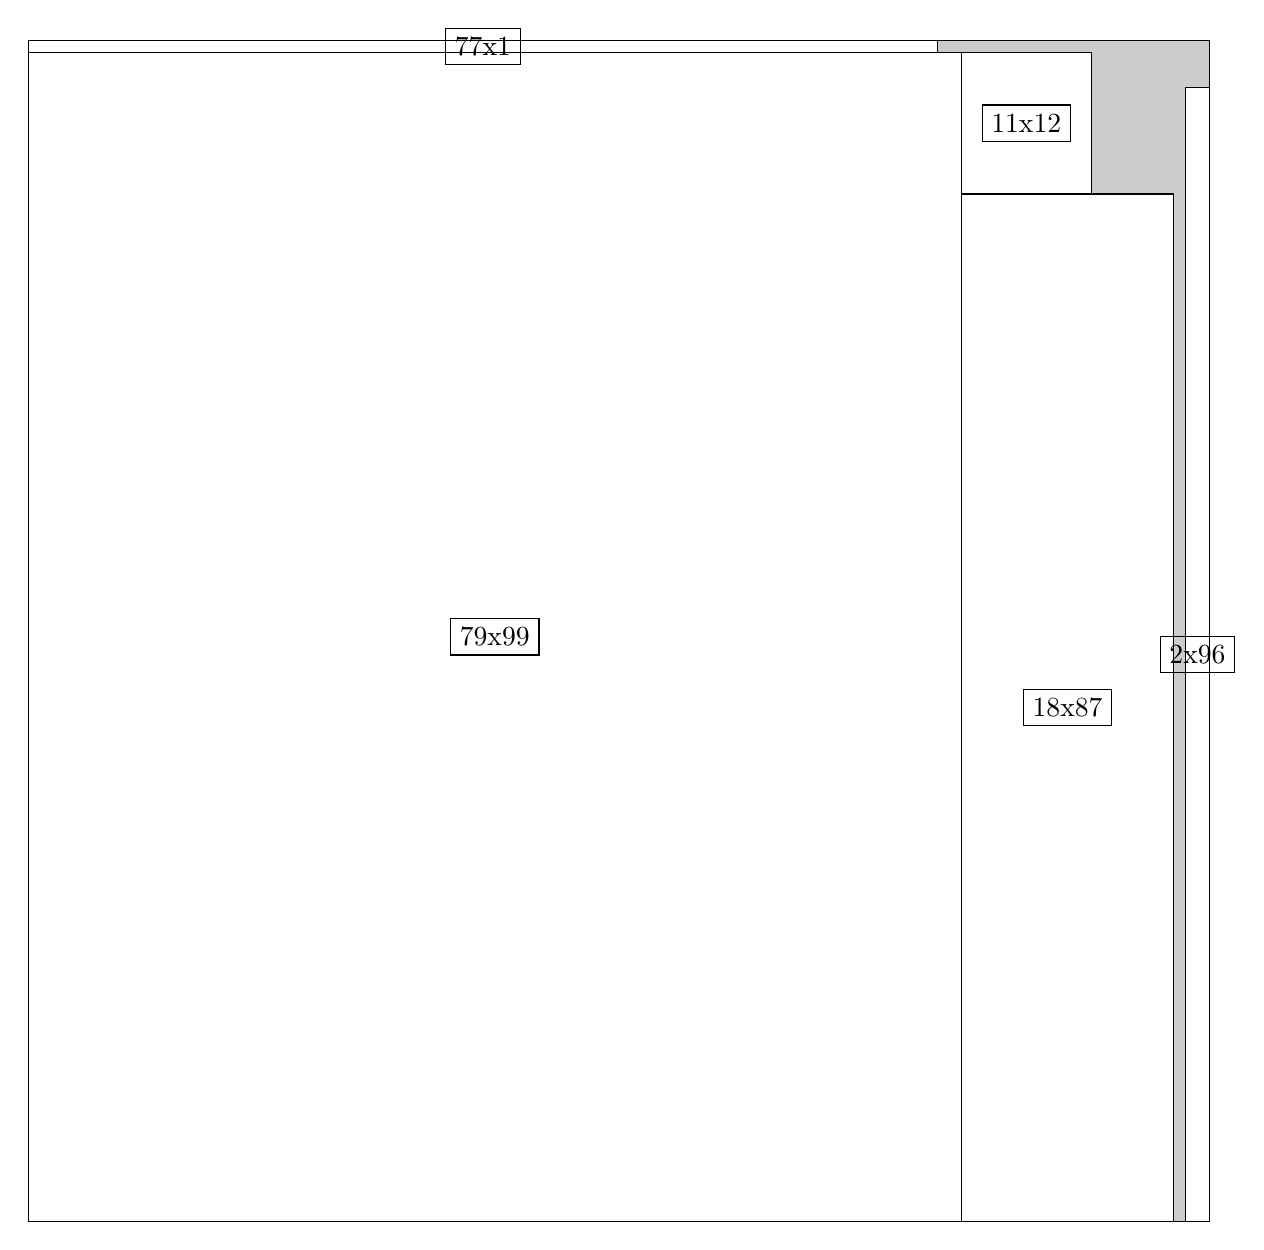
\begin{tikzpicture}[shorten >=1pt,scale=1.0,every node/.style={scale=1.0},->]
\tikzstyle{vertex}=[circle,fill=black!25,minimum size=14pt,inner sep=0pt]
\filldraw[fill=gray!40!white, draw=black] (0,0) rectangle (15.0,15.0);
\foreach \name/\x/\y/\w/\h in {79x99/0.0/0.0/11.85/14.85,18x87/11.85/0.0/2.6999999999999997/13.049999999999999,2x96/14.7/0.0/0.3/14.399999999999999,11x12/11.85/13.049999999999999/1.65/1.7999999999999998,77x1/0.0/14.85/11.549999999999999/0.15}
\filldraw[fill=white!40!white, draw=black] (\x,\y) rectangle node[draw] (\name) {\name} ++(\w,\h);
\end{tikzpicture}


w =79 , h =99 , x =0 , y =0 , v =7821
\par
w =18 , h =87 , x =79 , y =0 , v =1566
\par
w =2 , h =96 , x =98 , y =0 , v =192
\par
w =11 , h =12 , x =79 , y =87 , v =132
\par
w =77 , h =1 , x =0 , y =99 , v =77
\par
\newpage


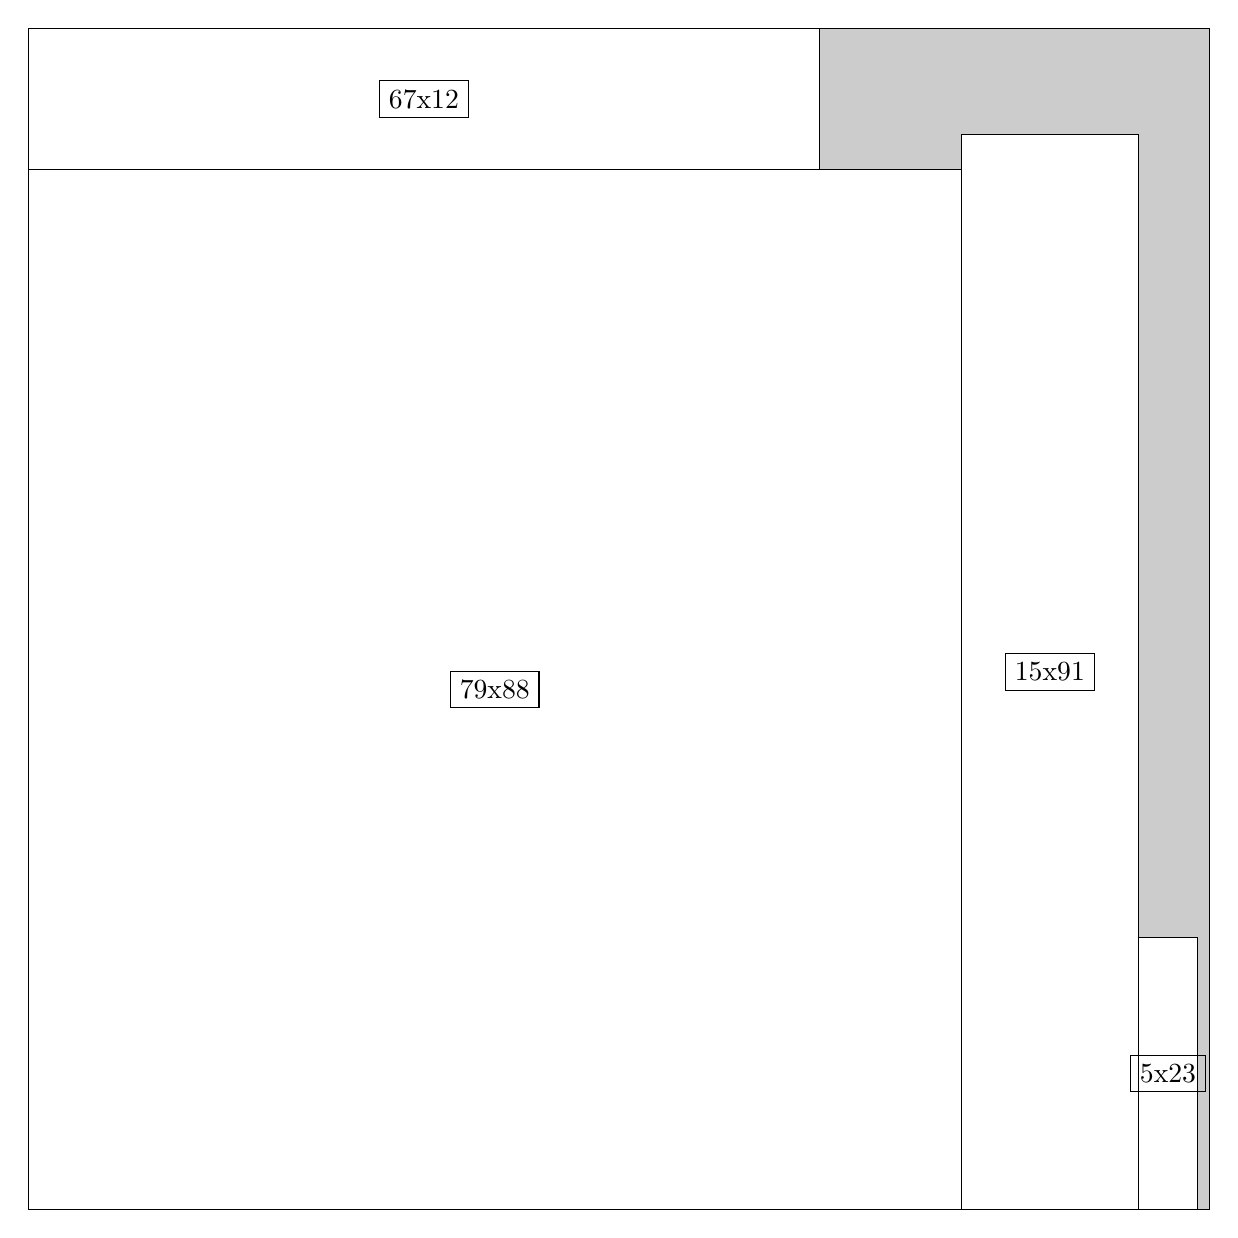
\begin{tikzpicture}[shorten >=1pt,scale=1.0,every node/.style={scale=1.0},->]
\tikzstyle{vertex}=[circle,fill=black!25,minimum size=14pt,inner sep=0pt]
\filldraw[fill=gray!40!white, draw=black] (0,0) rectangle (15.0,15.0);
\foreach \name/\x/\y/\w/\h in {79x88/0.0/0.0/11.85/13.2,15x91/11.85/0.0/2.25/13.65,67x12/0.0/13.2/10.049999999999999/1.7999999999999998,5x23/14.1/0.0/0.75/3.4499999999999997}
\filldraw[fill=white!40!white, draw=black] (\x,\y) rectangle node[draw] (\name) {\name} ++(\w,\h);
\end{tikzpicture}


w =79 , h =88 , x =0 , y =0 , v =6952
\par
w =15 , h =91 , x =79 , y =0 , v =1365
\par
w =67 , h =12 , x =0 , y =88 , v =804
\par
w =5 , h =23 , x =94 , y =0 , v =115
\par
\newpage


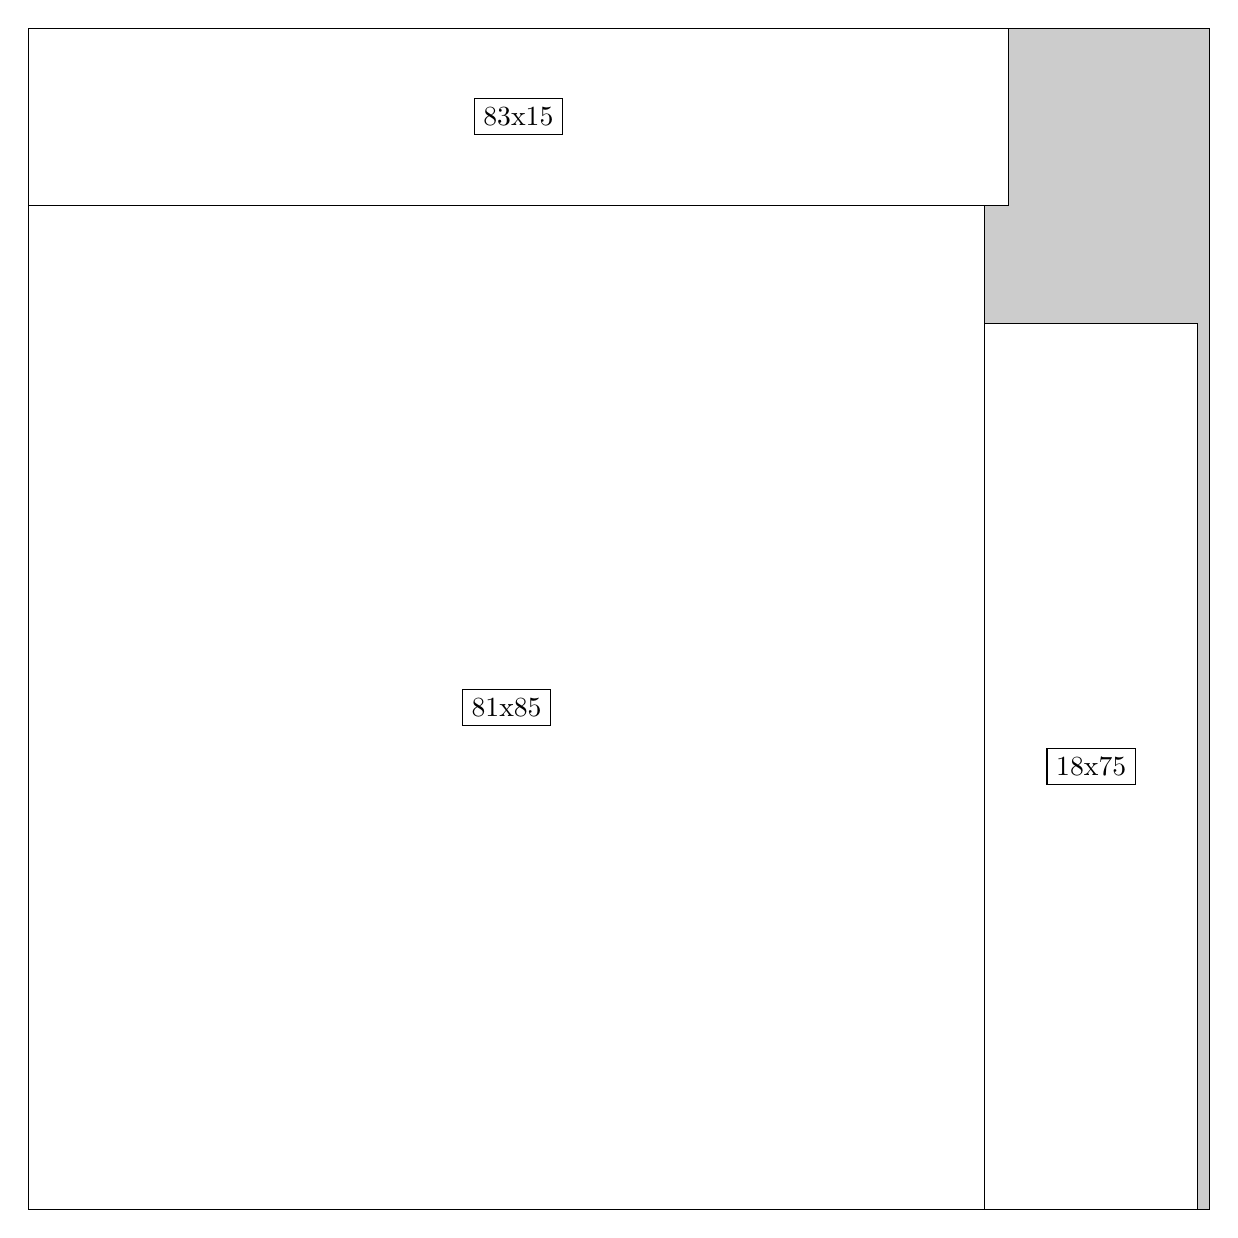
\begin{tikzpicture}[shorten >=1pt,scale=1.0,every node/.style={scale=1.0},->]
\tikzstyle{vertex}=[circle,fill=black!25,minimum size=14pt,inner sep=0pt]
\filldraw[fill=gray!40!white, draw=black] (0,0) rectangle (15.0,15.0);
\foreach \name/\x/\y/\w/\h in {81x85/0.0/0.0/12.15/12.75,18x75/12.15/0.0/2.6999999999999997/11.25,83x15/0.0/12.75/12.45/2.25}
\filldraw[fill=white!40!white, draw=black] (\x,\y) rectangle node[draw] (\name) {\name} ++(\w,\h);
\end{tikzpicture}


w =81 , h =85 , x =0 , y =0 , v =6885
\par
w =18 , h =75 , x =81 , y =0 , v =1350
\par
w =83 , h =15 , x =0 , y =85 , v =1245
\par
\newpage


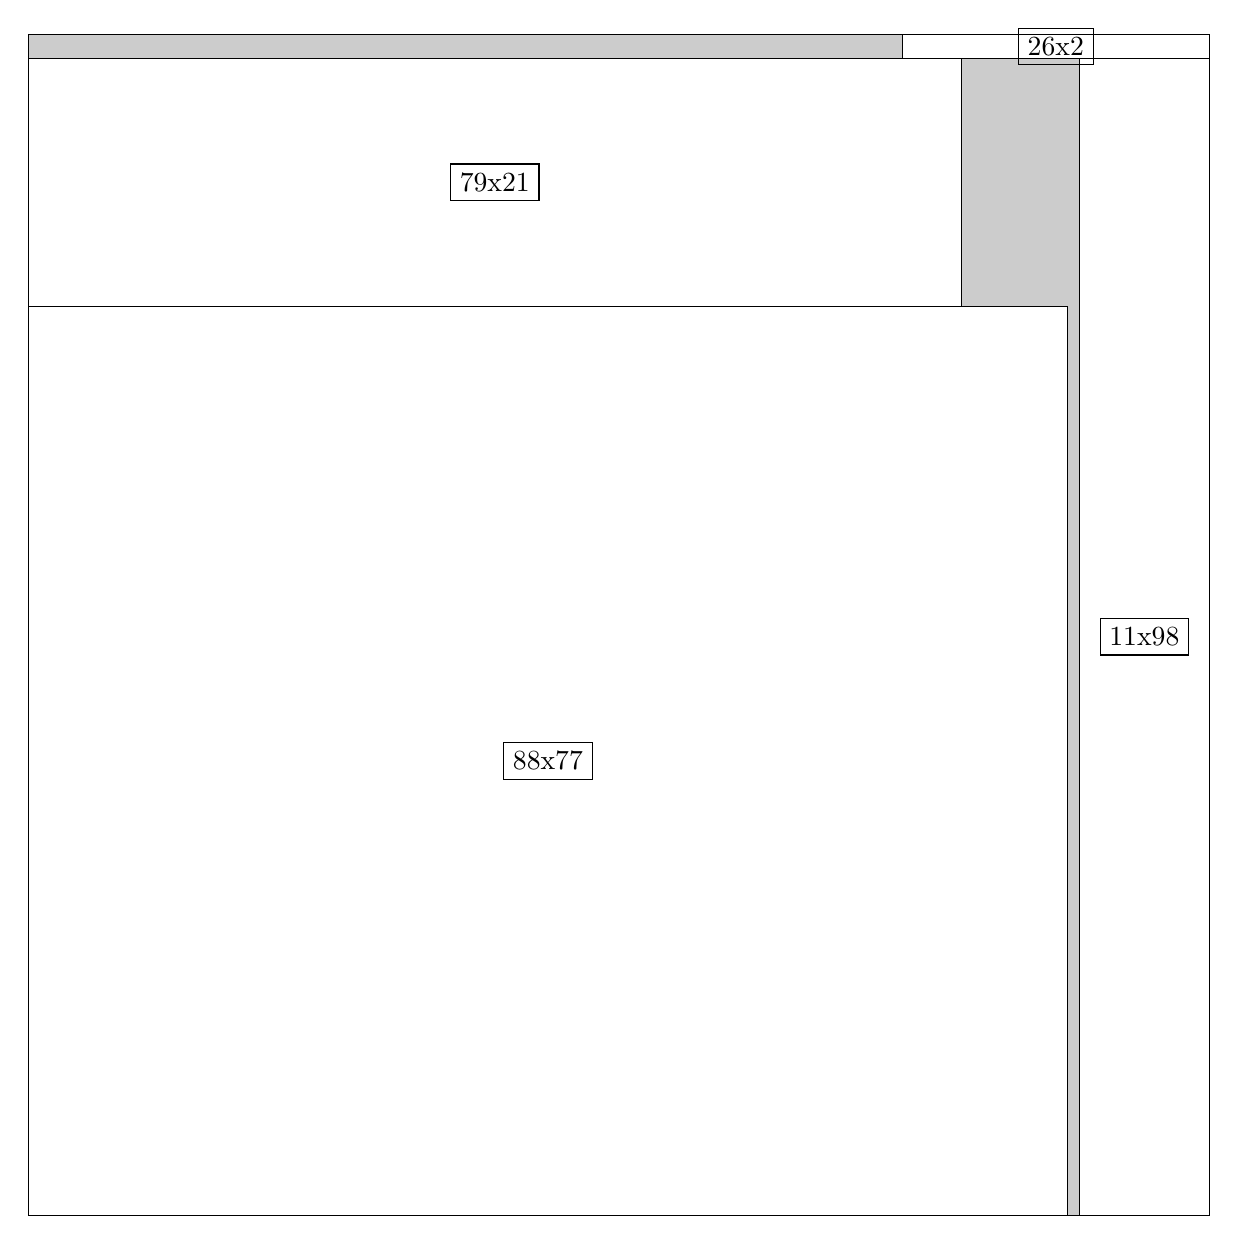
\begin{tikzpicture}[shorten >=1pt,scale=1.0,every node/.style={scale=1.0},->]
\tikzstyle{vertex}=[circle,fill=black!25,minimum size=14pt,inner sep=0pt]
\filldraw[fill=gray!40!white, draw=black] (0,0) rectangle (15.0,15.0);
\foreach \name/\x/\y/\w/\h in {88x77/0.0/0.0/13.2/11.549999999999999,11x98/13.35/0.0/1.65/14.7,79x21/0.0/11.549999999999999/11.85/3.15,26x2/11.1/14.7/3.9/0.3}
\filldraw[fill=white!40!white, draw=black] (\x,\y) rectangle node[draw] (\name) {\name} ++(\w,\h);
\end{tikzpicture}


w =88 , h =77 , x =0 , y =0 , v =6776
\par
w =11 , h =98 , x =89 , y =0 , v =1078
\par
w =79 , h =21 , x =0 , y =77 , v =1659
\par
w =26 , h =2 , x =74 , y =98 , v =52
\par
\newpage


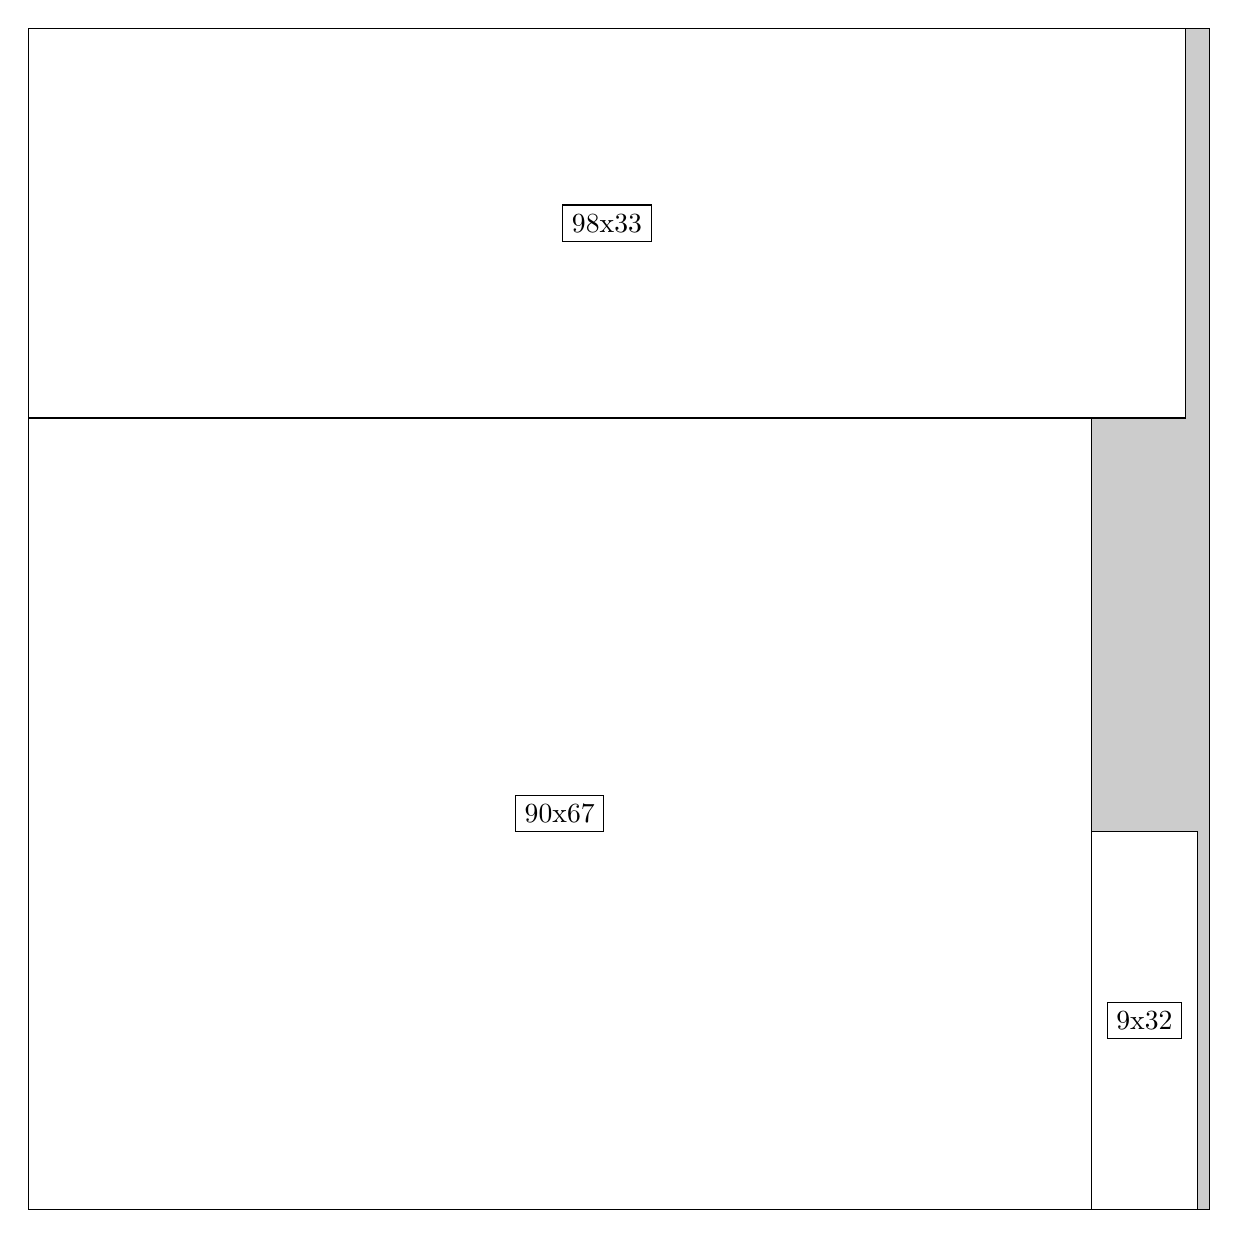
\begin{tikzpicture}[shorten >=1pt,scale=1.0,every node/.style={scale=1.0},->]
\tikzstyle{vertex}=[circle,fill=black!25,minimum size=14pt,inner sep=0pt]
\filldraw[fill=gray!40!white, draw=black] (0,0) rectangle (15.0,15.0);
\foreach \name/\x/\y/\w/\h in {90x67/0.0/0.0/13.5/10.049999999999999,98x33/0.0/10.049999999999999/14.7/4.95,9x32/13.5/0.0/1.3499999999999999/4.8}
\filldraw[fill=white!40!white, draw=black] (\x,\y) rectangle node[draw] (\name) {\name} ++(\w,\h);
\end{tikzpicture}


w =90 , h =67 , x =0 , y =0 , v =6030
\par
w =98 , h =33 , x =0 , y =67 , v =3234
\par
w =9 , h =32 , x =90 , y =0 , v =288
\par
\newpage


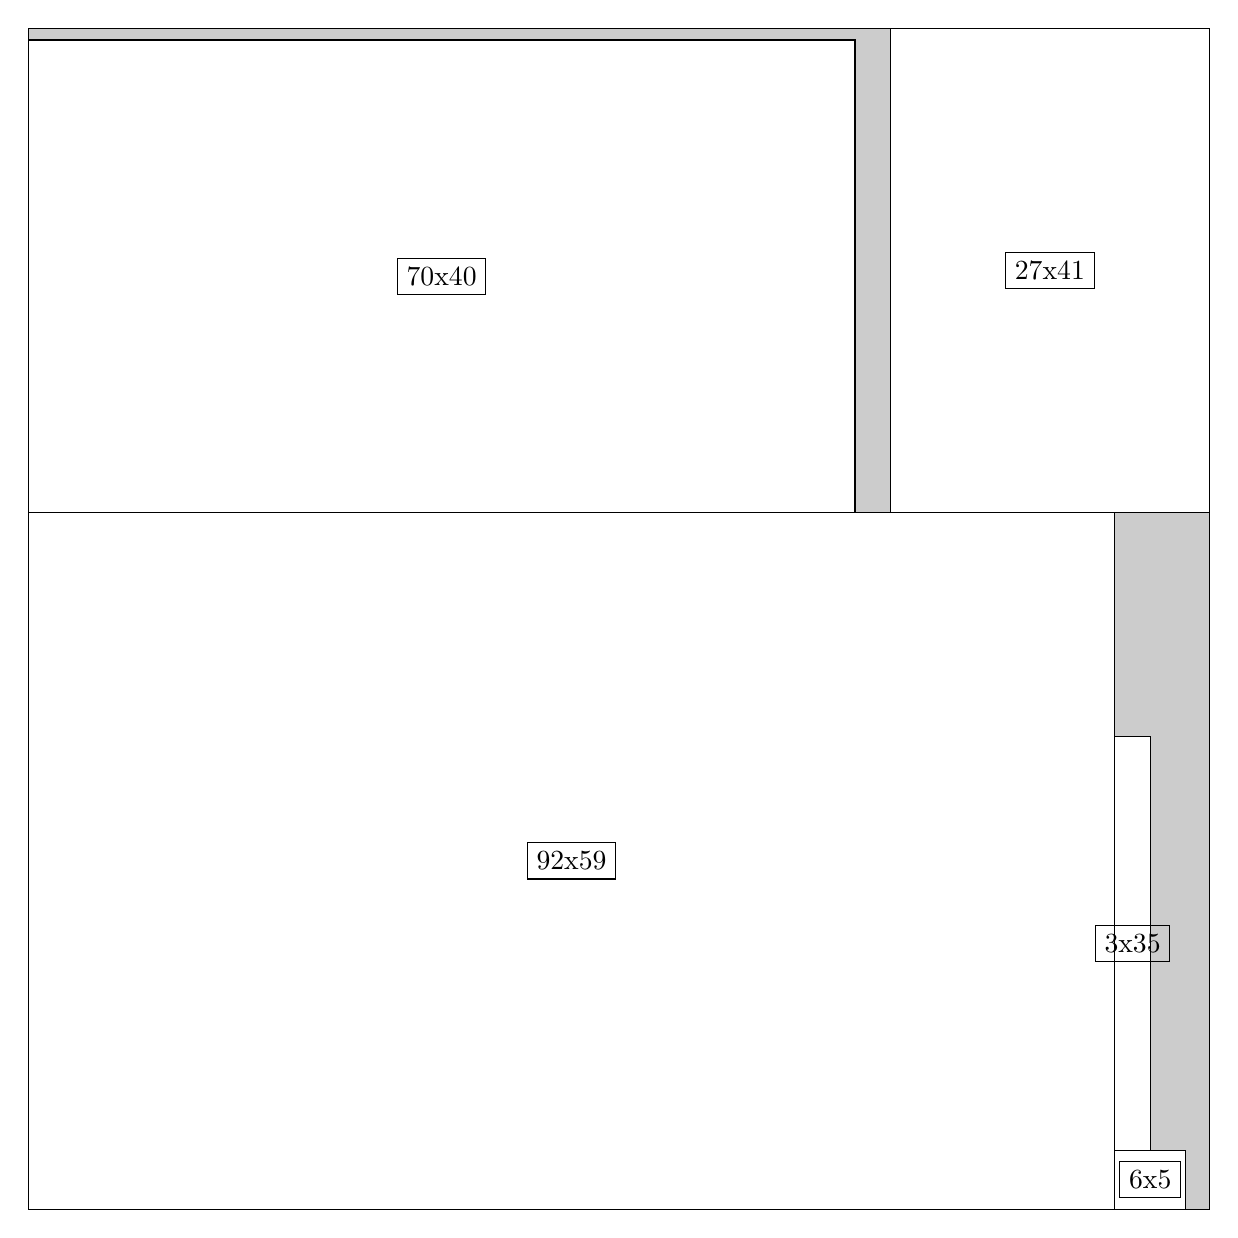
\begin{tikzpicture}[shorten >=1pt,scale=1.0,every node/.style={scale=1.0},->]
\tikzstyle{vertex}=[circle,fill=black!25,minimum size=14pt,inner sep=0pt]
\filldraw[fill=gray!40!white, draw=black] (0,0) rectangle (15.0,15.0);
\foreach \name/\x/\y/\w/\h in {92x59/0.0/0.0/13.799999999999999/8.85,70x40/0.0/8.85/10.5/6.0,27x41/10.95/8.85/4.05/6.1499999999999995,3x35/13.799999999999999/0.75/0.44999999999999996/5.25,6x5/13.799999999999999/0.0/0.8999999999999999/0.75}
\filldraw[fill=white!40!white, draw=black] (\x,\y) rectangle node[draw] (\name) {\name} ++(\w,\h);
\end{tikzpicture}


w =92 , h =59 , x =0 , y =0 , v =5428
\par
w =70 , h =40 , x =0 , y =59 , v =2800
\par
w =27 , h =41 , x =73 , y =59 , v =1107
\par
w =3 , h =35 , x =92 , y =5 , v =105
\par
w =6 , h =5 , x =92 , y =0 , v =30
\par
\newpage


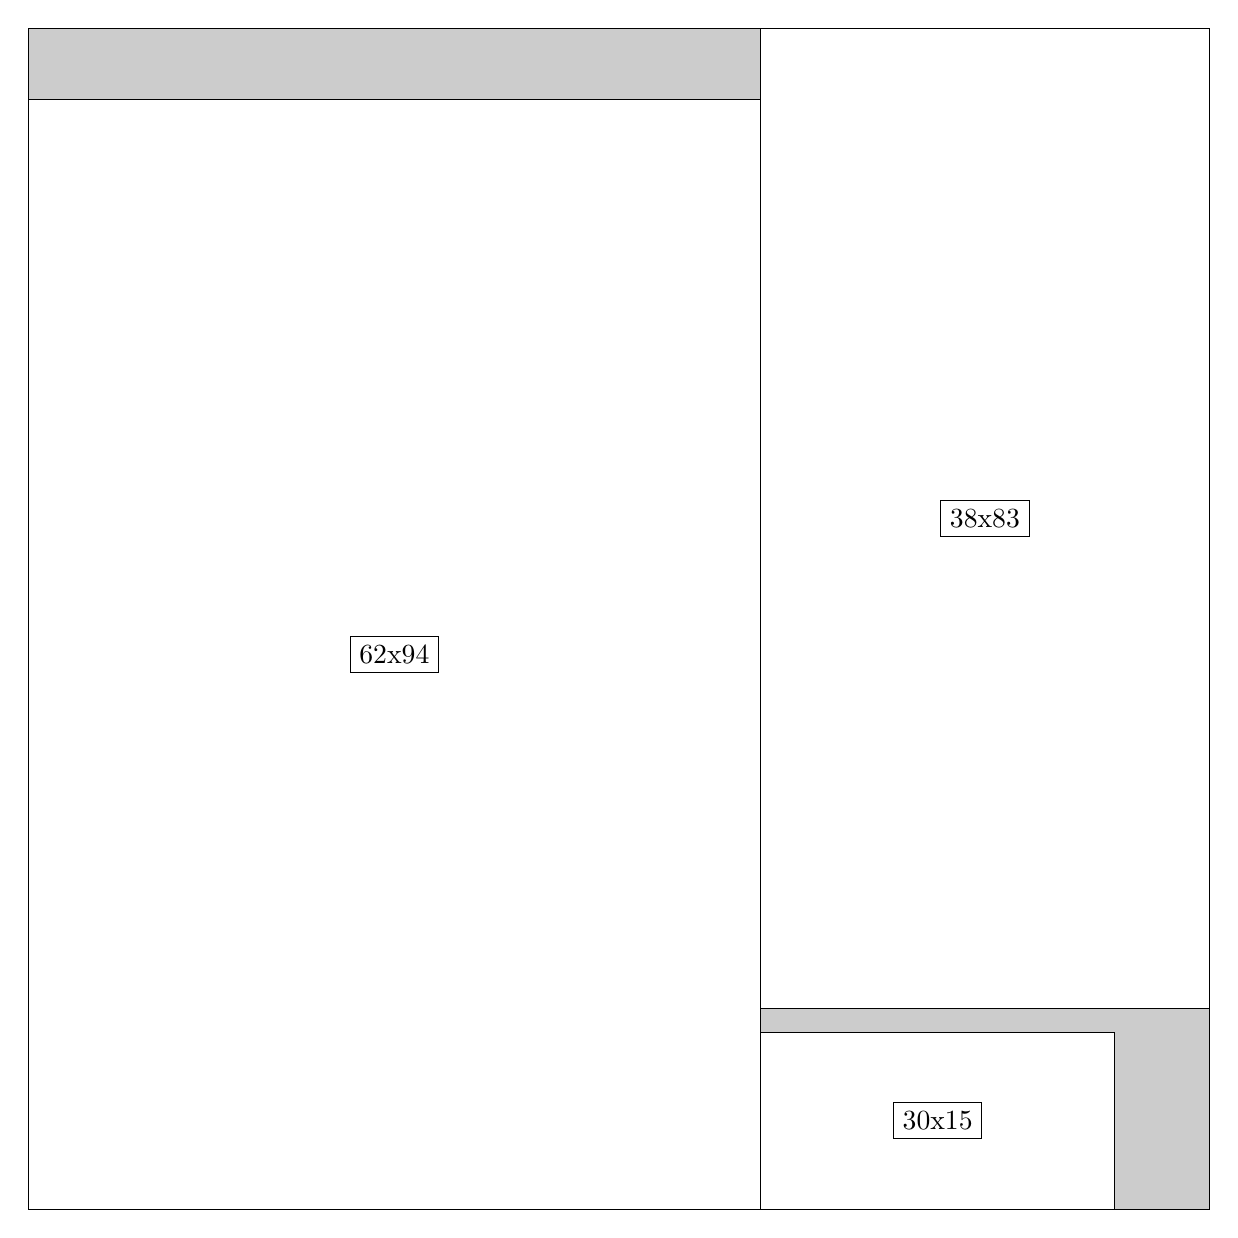
\begin{tikzpicture}[shorten >=1pt,scale=1.0,every node/.style={scale=1.0},->]
\tikzstyle{vertex}=[circle,fill=black!25,minimum size=14pt,inner sep=0pt]
\filldraw[fill=gray!40!white, draw=black] (0,0) rectangle (15.0,15.0);
\foreach \name/\x/\y/\w/\h in {38x83/9.299999999999999/2.55/5.7/12.45,62x94/0.0/0.0/9.299999999999999/14.1,30x15/9.299999999999999/0.0/4.5/2.25}
\filldraw[fill=white!40!white, draw=black] (\x,\y) rectangle node[draw] (\name) {\name} ++(\w,\h);
\end{tikzpicture}


w =38 , h =83 , x =62 , y =17 , v =3154
\par
w =62 , h =94 , x =0 , y =0 , v =5828
\par
w =30 , h =15 , x =62 , y =0 , v =450
\par
\newpage


\begin{tikzpicture}[shorten >=1pt,scale=1.0,every node/.style={scale=1.0},->]
\tikzstyle{vertex}=[circle,fill=black!25,minimum size=14pt,inner sep=0pt]
\filldraw[fill=gray!40!white, draw=black] (0,0) rectangle (15.0,15.0);
\foreach \name/\x/\y/\w/\h in {61x89/0.0/0.0/9.15/13.35,39x78/9.15/0.0/5.85/11.7,38x22/9.299999999999999/11.7/5.7/3.3,57x11/0.0/13.35/8.549999999999999/1.65}
\filldraw[fill=white!40!white, draw=black] (\x,\y) rectangle node[draw] (\name) {\name} ++(\w,\h);
\end{tikzpicture}


w =61 , h =89 , x =0 , y =0 , v =5429
\par
w =39 , h =78 , x =61 , y =0 , v =3042
\par
w =38 , h =22 , x =62 , y =78 , v =836
\par
w =57 , h =11 , x =0 , y =89 , v =627
\par
\newpage


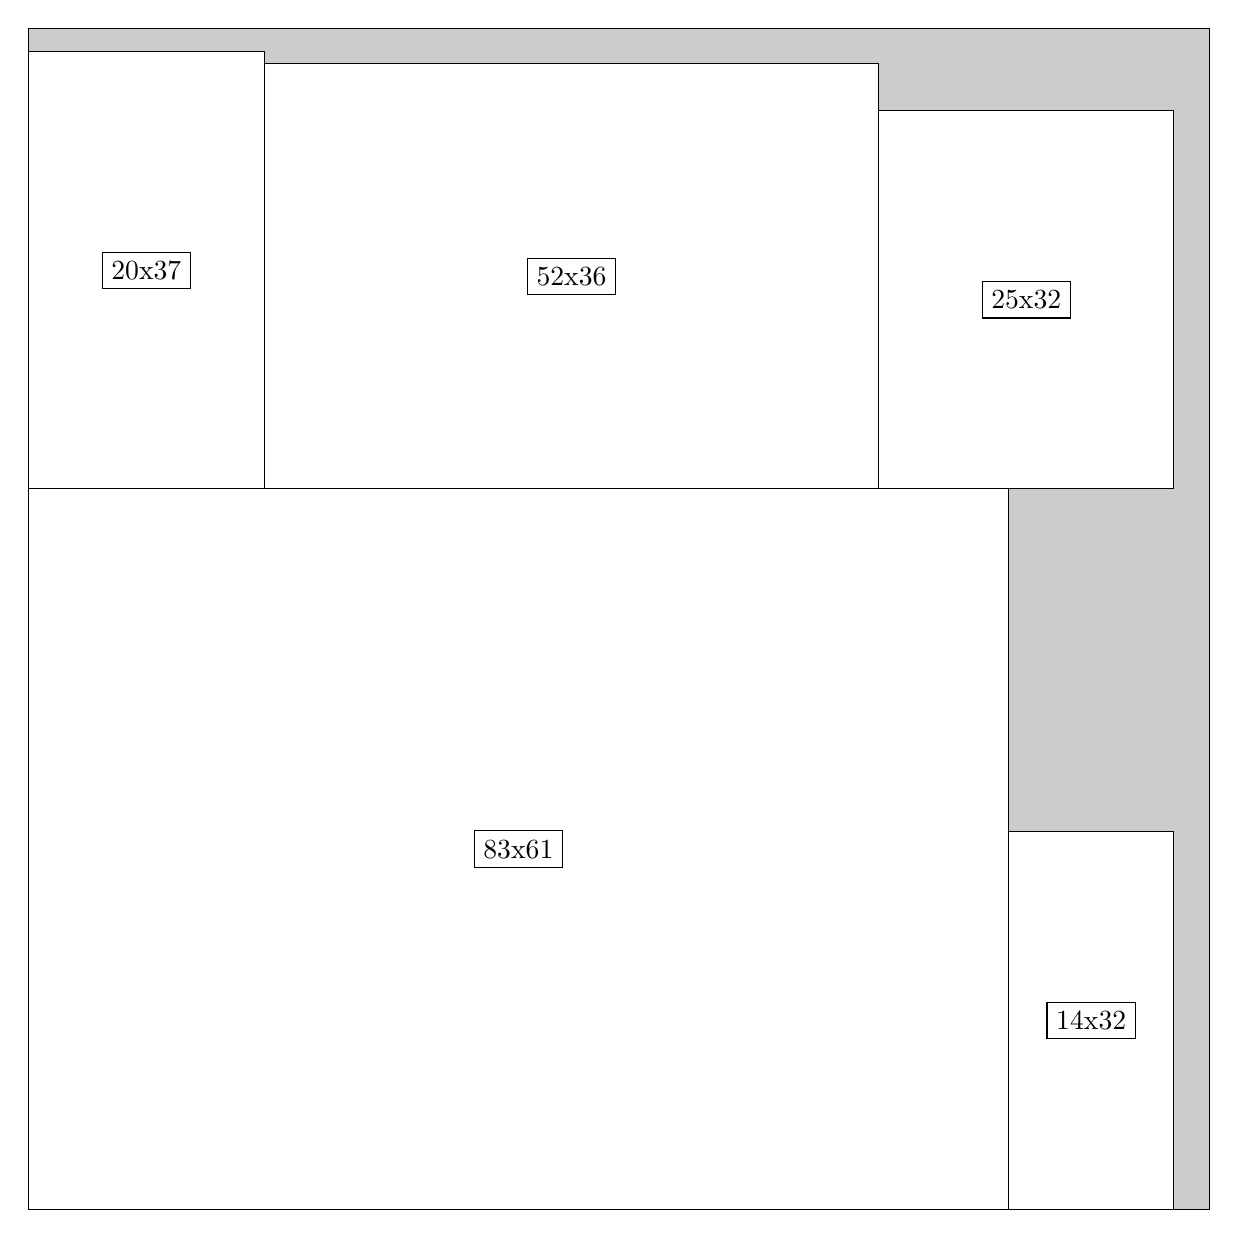
\begin{tikzpicture}[shorten >=1pt,scale=1.0,every node/.style={scale=1.0},->]
\tikzstyle{vertex}=[circle,fill=black!25,minimum size=14pt,inner sep=0pt]
\filldraw[fill=gray!40!white, draw=black] (0,0) rectangle (15.0,15.0);
\foreach \name/\x/\y/\w/\h in {83x61/0.0/0.0/12.45/9.15,52x36/3.0/9.15/7.8/5.3999999999999995,25x32/10.799999999999999/9.15/3.75/4.8,20x37/0.0/9.15/3.0/5.55,14x32/12.45/0.0/2.1/4.8}
\filldraw[fill=white!40!white, draw=black] (\x,\y) rectangle node[draw] (\name) {\name} ++(\w,\h);
\end{tikzpicture}


w =83 , h =61 , x =0 , y =0 , v =5063
\par
w =52 , h =36 , x =20 , y =61 , v =1872
\par
w =25 , h =32 , x =72 , y =61 , v =800
\par
w =20 , h =37 , x =0 , y =61 , v =740
\par
w =14 , h =32 , x =83 , y =0 , v =448
\par
\newpage


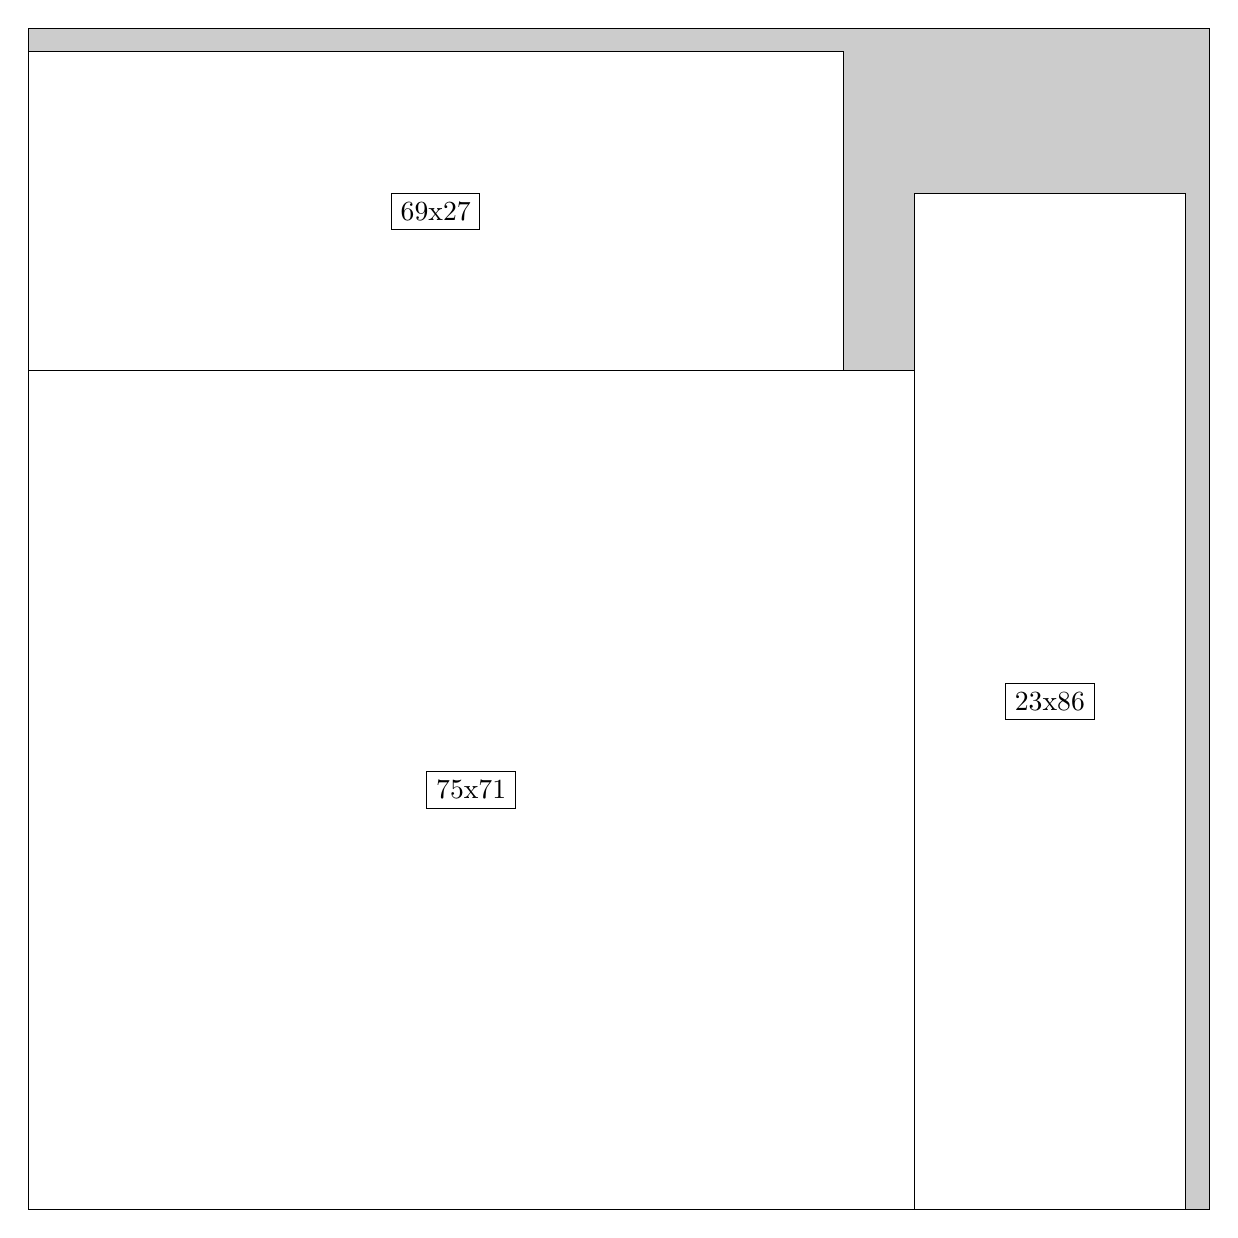
\begin{tikzpicture}[shorten >=1pt,scale=1.0,every node/.style={scale=1.0},->]
\tikzstyle{vertex}=[circle,fill=black!25,minimum size=14pt,inner sep=0pt]
\filldraw[fill=gray!40!white, draw=black] (0,0) rectangle (15.0,15.0);
\foreach \name/\x/\y/\w/\h in {75x71/0.0/0.0/11.25/10.65,23x86/11.25/0.0/3.4499999999999997/12.9,69x27/0.0/10.65/10.35/4.05}
\filldraw[fill=white!40!white, draw=black] (\x,\y) rectangle node[draw] (\name) {\name} ++(\w,\h);
\end{tikzpicture}


w =75 , h =71 , x =0 , y =0 , v =5325
\par
w =23 , h =86 , x =75 , y =0 , v =1978
\par
w =69 , h =27 , x =0 , y =71 , v =1863
\par
\newpage


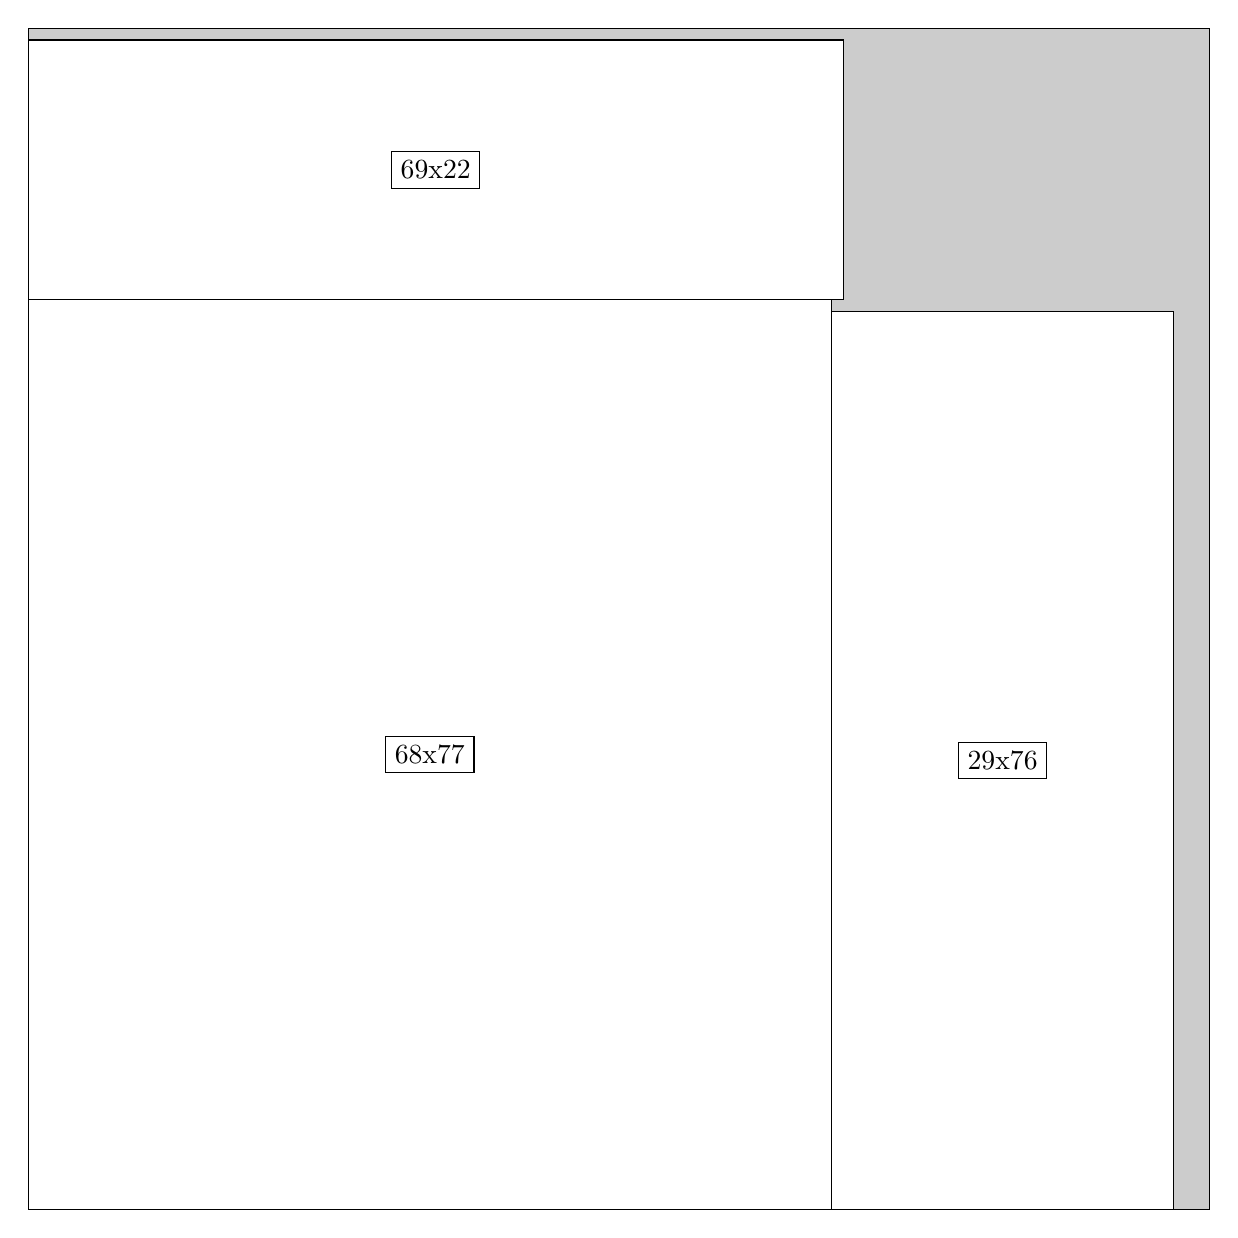
\begin{tikzpicture}[shorten >=1pt,scale=1.0,every node/.style={scale=1.0},->]
\tikzstyle{vertex}=[circle,fill=black!25,minimum size=14pt,inner sep=0pt]
\filldraw[fill=gray!40!white, draw=black] (0,0) rectangle (15.0,15.0);
\foreach \name/\x/\y/\w/\h in {68x77/0.0/0.0/10.2/11.549999999999999,29x76/10.2/0.0/4.35/11.4,69x22/0.0/11.549999999999999/10.35/3.3}
\filldraw[fill=white!40!white, draw=black] (\x,\y) rectangle node[draw] (\name) {\name} ++(\w,\h);
\end{tikzpicture}


w =68 , h =77 , x =0 , y =0 , v =5236
\par
w =29 , h =76 , x =68 , y =0 , v =2204
\par
w =69 , h =22 , x =0 , y =77 , v =1518
\par
\newpage


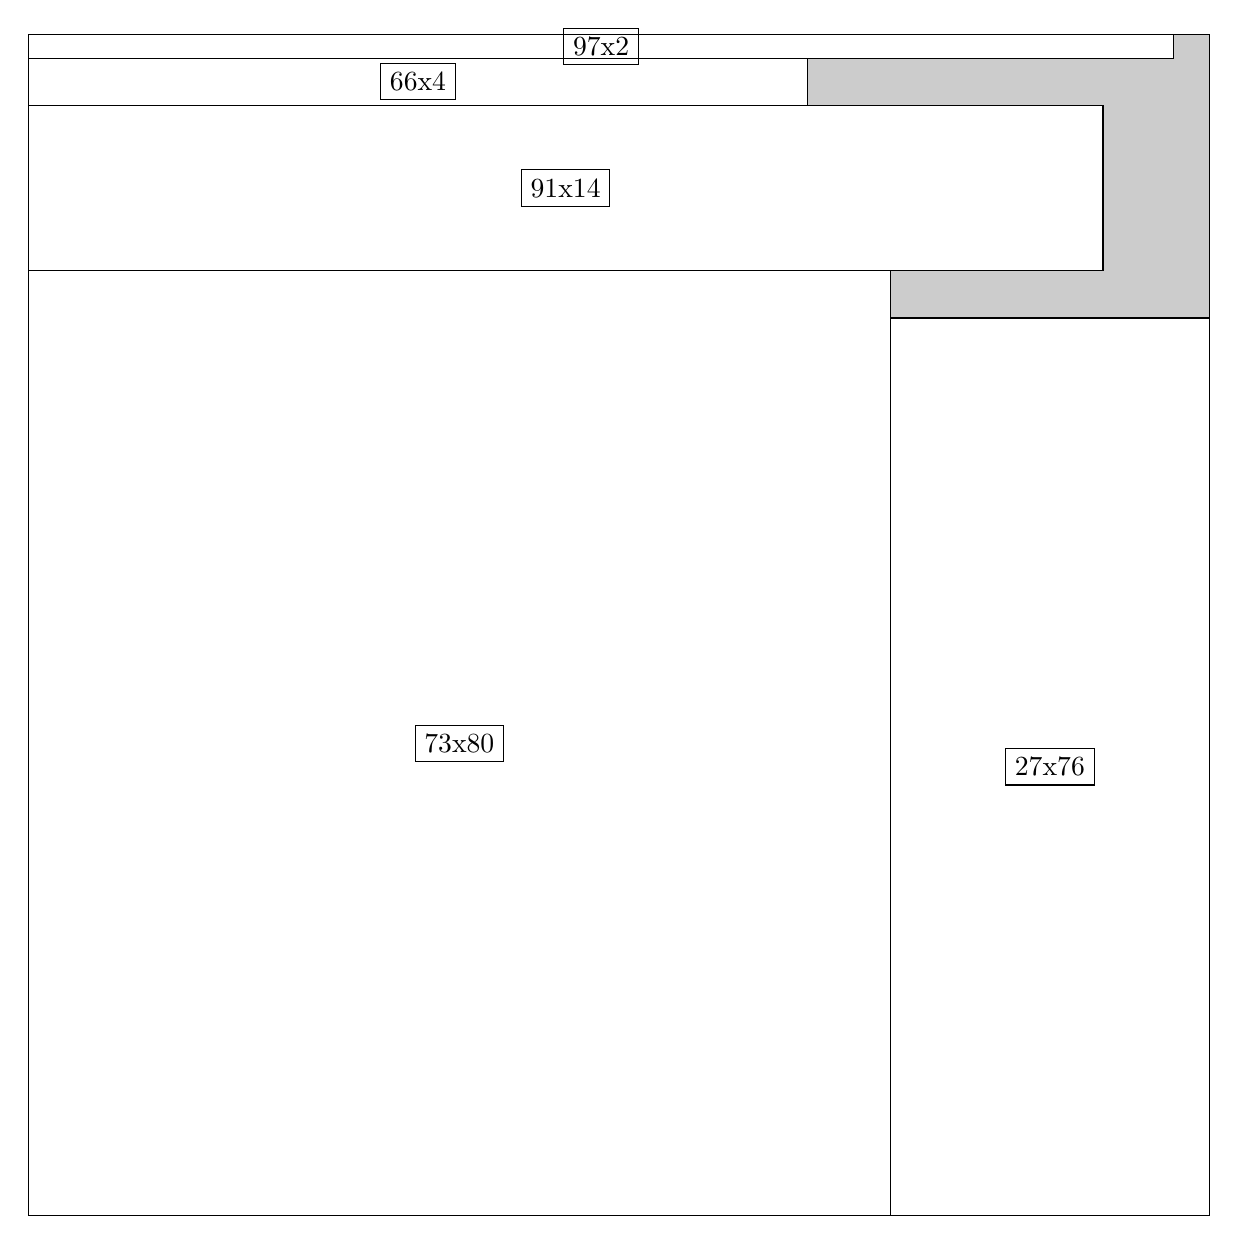
\begin{tikzpicture}[shorten >=1pt,scale=1.0,every node/.style={scale=1.0},->]
\tikzstyle{vertex}=[circle,fill=black!25,minimum size=14pt,inner sep=0pt]
\filldraw[fill=gray!40!white, draw=black] (0,0) rectangle (15.0,15.0);
\foreach \name/\x/\y/\w/\h in {73x80/0.0/0.0/10.95/12.0,27x76/10.95/0.0/4.05/11.4,91x14/0.0/12.0/13.65/2.1,66x4/0.0/14.1/9.9/0.6,97x2/0.0/14.7/14.549999999999999/0.3}
\filldraw[fill=white!40!white, draw=black] (\x,\y) rectangle node[draw] (\name) {\name} ++(\w,\h);
\end{tikzpicture}


w =73 , h =80 , x =0 , y =0 , v =5840
\par
w =27 , h =76 , x =73 , y =0 , v =2052
\par
w =91 , h =14 , x =0 , y =80 , v =1274
\par
w =66 , h =4 , x =0 , y =94 , v =264
\par
w =97 , h =2 , x =0 , y =98 , v =194
\par
\newpage


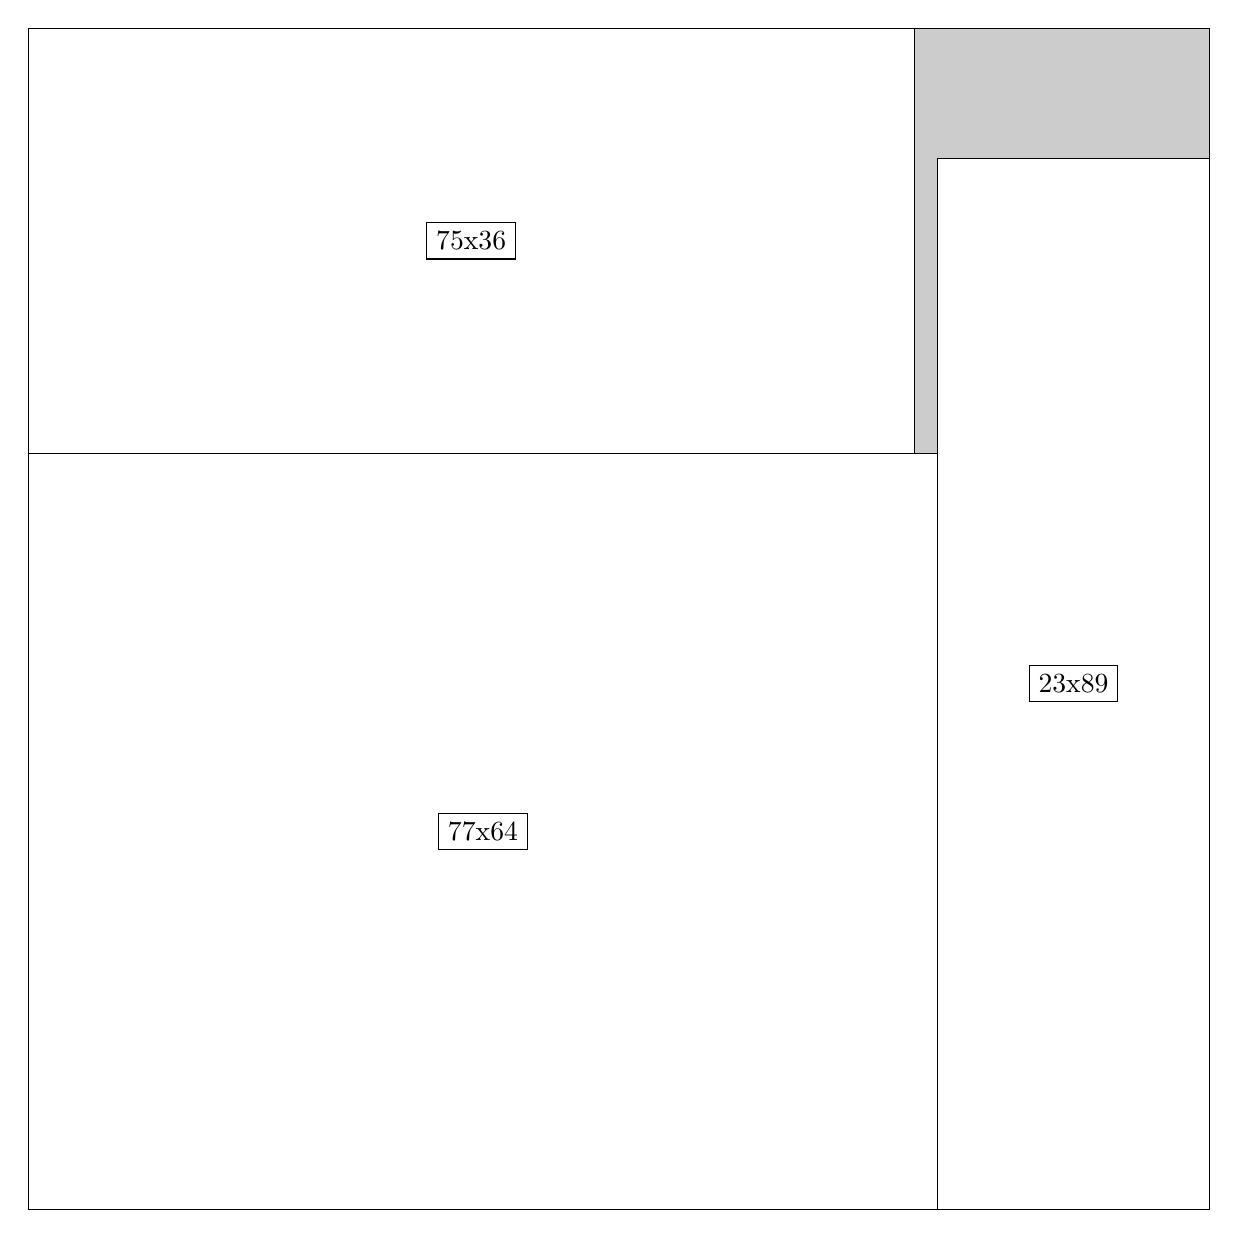
\begin{tikzpicture}[shorten >=1pt,scale=1.0,every node/.style={scale=1.0},->]
\tikzstyle{vertex}=[circle,fill=black!25,minimum size=14pt,inner sep=0pt]
\filldraw[fill=gray!40!white, draw=black] (0,0) rectangle (15.0,15.0);
\foreach \name/\x/\y/\w/\h in {77x64/0.0/0.0/11.549999999999999/9.6,75x36/0.0/9.6/11.25/5.3999999999999995,23x89/11.549999999999999/0.0/3.4499999999999997/13.35}
\filldraw[fill=white!40!white, draw=black] (\x,\y) rectangle node[draw] (\name) {\name} ++(\w,\h);
\end{tikzpicture}


w =77 , h =64 , x =0 , y =0 , v =4928
\par
w =75 , h =36 , x =0 , y =64 , v =2700
\par
w =23 , h =89 , x =77 , y =0 , v =2047
\par
\newpage


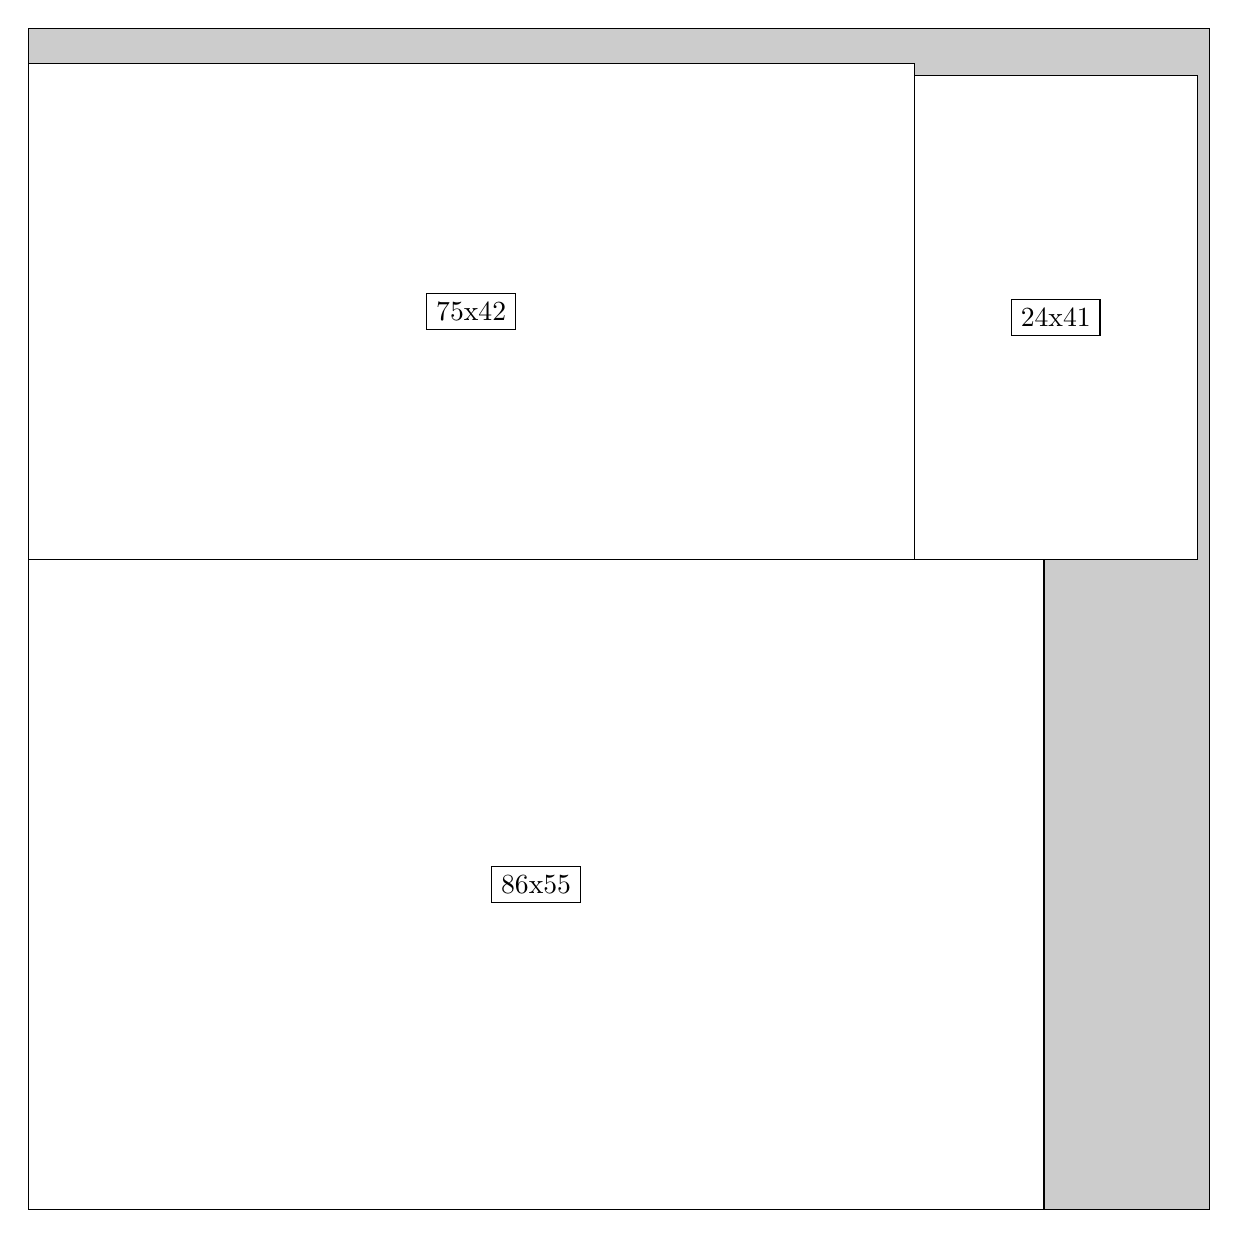
\begin{tikzpicture}[shorten >=1pt,scale=1.0,every node/.style={scale=1.0},->]
\tikzstyle{vertex}=[circle,fill=black!25,minimum size=14pt,inner sep=0pt]
\filldraw[fill=gray!40!white, draw=black] (0,0) rectangle (15.0,15.0);
\foreach \name/\x/\y/\w/\h in {86x55/0.0/0.0/12.9/8.25,75x42/0.0/8.25/11.25/6.3,24x41/11.25/8.25/3.5999999999999996/6.1499999999999995}
\filldraw[fill=white!40!white, draw=black] (\x,\y) rectangle node[draw] (\name) {\name} ++(\w,\h);
\end{tikzpicture}


w =86 , h =55 , x =0 , y =0 , v =4730
\par
w =75 , h =42 , x =0 , y =55 , v =3150
\par
w =24 , h =41 , x =75 , y =55 , v =984
\par
\newpage


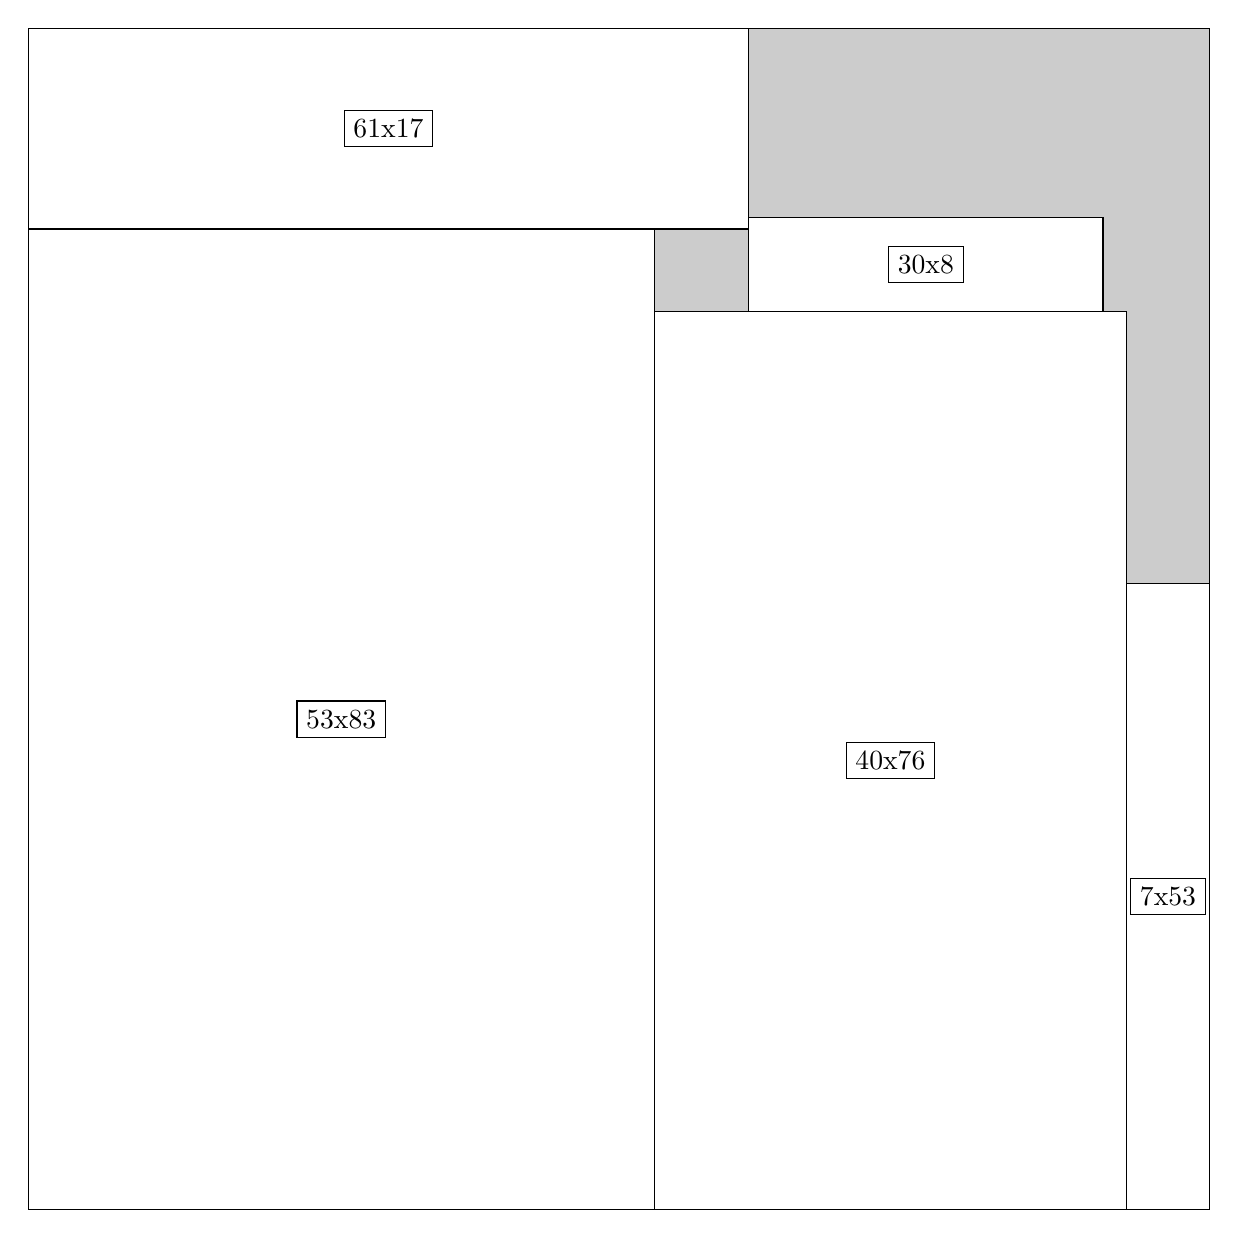
\begin{tikzpicture}[shorten >=1pt,scale=1.0,every node/.style={scale=1.0},->]
\tikzstyle{vertex}=[circle,fill=black!25,minimum size=14pt,inner sep=0pt]
\filldraw[fill=gray!40!white, draw=black] (0,0) rectangle (15.0,15.0);
\foreach \name/\x/\y/\w/\h in {53x83/0.0/0.0/7.949999999999999/12.45,40x76/7.949999999999999/0.0/6.0/11.4,61x17/0.0/12.45/9.15/2.55,7x53/13.95/0.0/1.05/7.949999999999999,30x8/9.15/11.4/4.5/1.2}
\filldraw[fill=white!40!white, draw=black] (\x,\y) rectangle node[draw] (\name) {\name} ++(\w,\h);
\end{tikzpicture}


w =53 , h =83 , x =0 , y =0 , v =4399
\par
w =40 , h =76 , x =53 , y =0 , v =3040
\par
w =61 , h =17 , x =0 , y =83 , v =1037
\par
w =7 , h =53 , x =93 , y =0 , v =371
\par
w =30 , h =8 , x =61 , y =76 , v =240
\par
\newpage


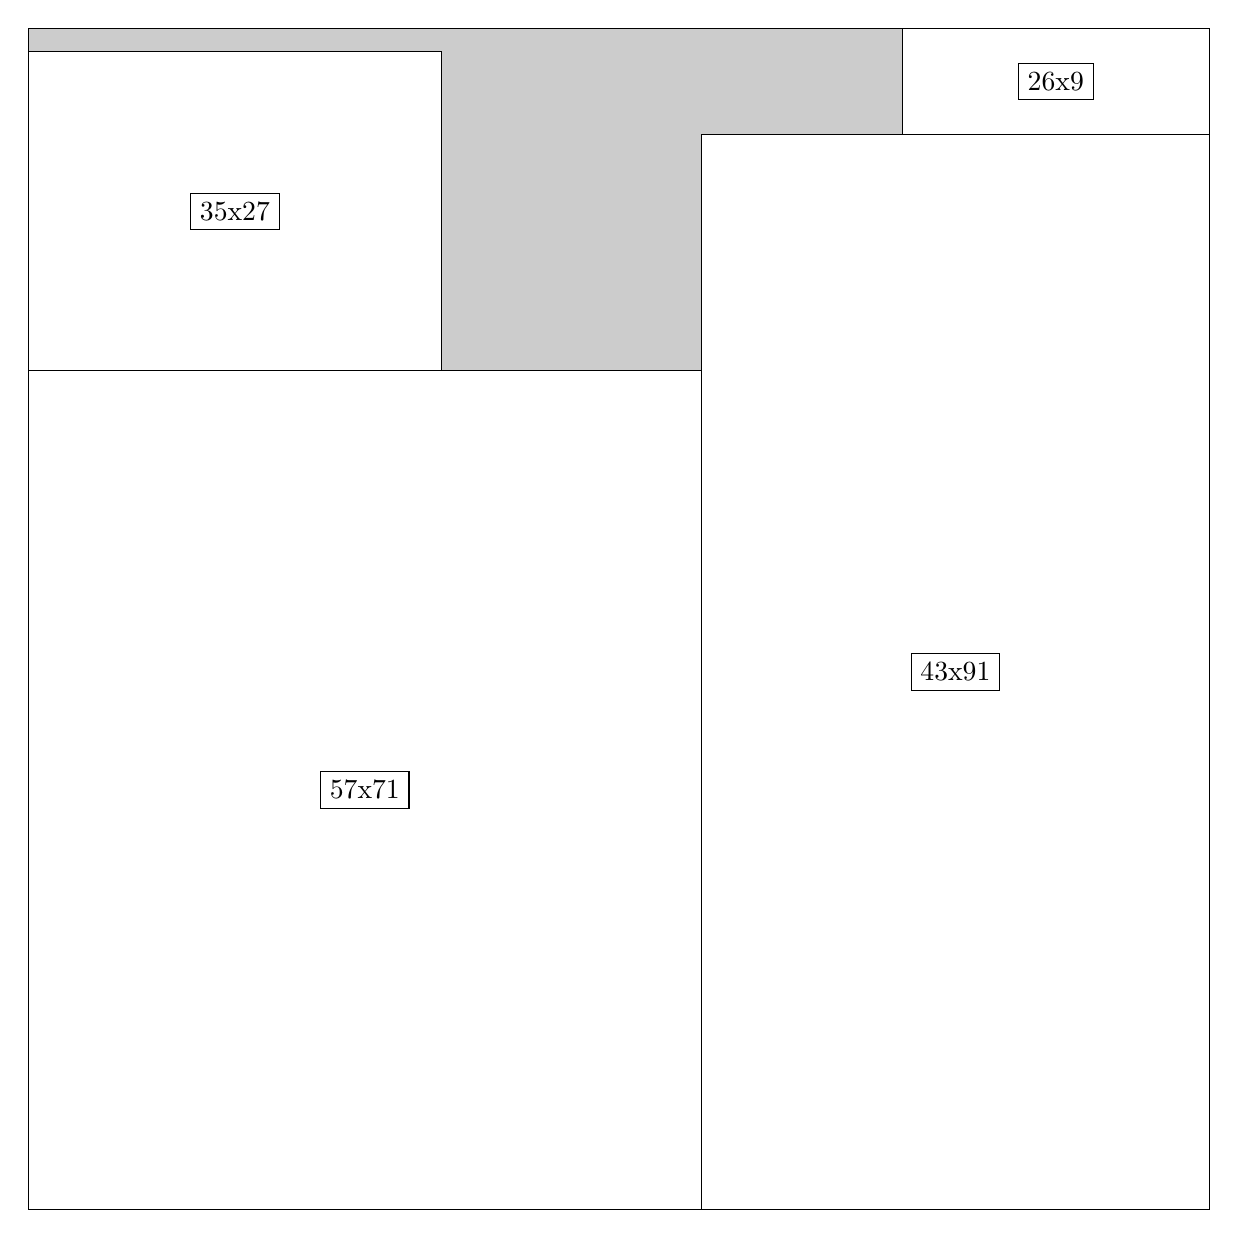
\begin{tikzpicture}[shorten >=1pt,scale=1.0,every node/.style={scale=1.0},->]
\tikzstyle{vertex}=[circle,fill=black!25,minimum size=14pt,inner sep=0pt]
\filldraw[fill=gray!40!white, draw=black] (0,0) rectangle (15.0,15.0);
\foreach \name/\x/\y/\w/\h in {57x71/0.0/0.0/8.549999999999999/10.65,43x91/8.549999999999999/0.0/6.45/13.65,35x27/0.0/10.65/5.25/4.05,26x9/11.1/13.65/3.9/1.3499999999999999}
\filldraw[fill=white!40!white, draw=black] (\x,\y) rectangle node[draw] (\name) {\name} ++(\w,\h);
\end{tikzpicture}


w =57 , h =71 , x =0 , y =0 , v =4047
\par
w =43 , h =91 , x =57 , y =0 , v =3913
\par
w =35 , h =27 , x =0 , y =71 , v =945
\par
w =26 , h =9 , x =74 , y =91 , v =234
\par
\newpage


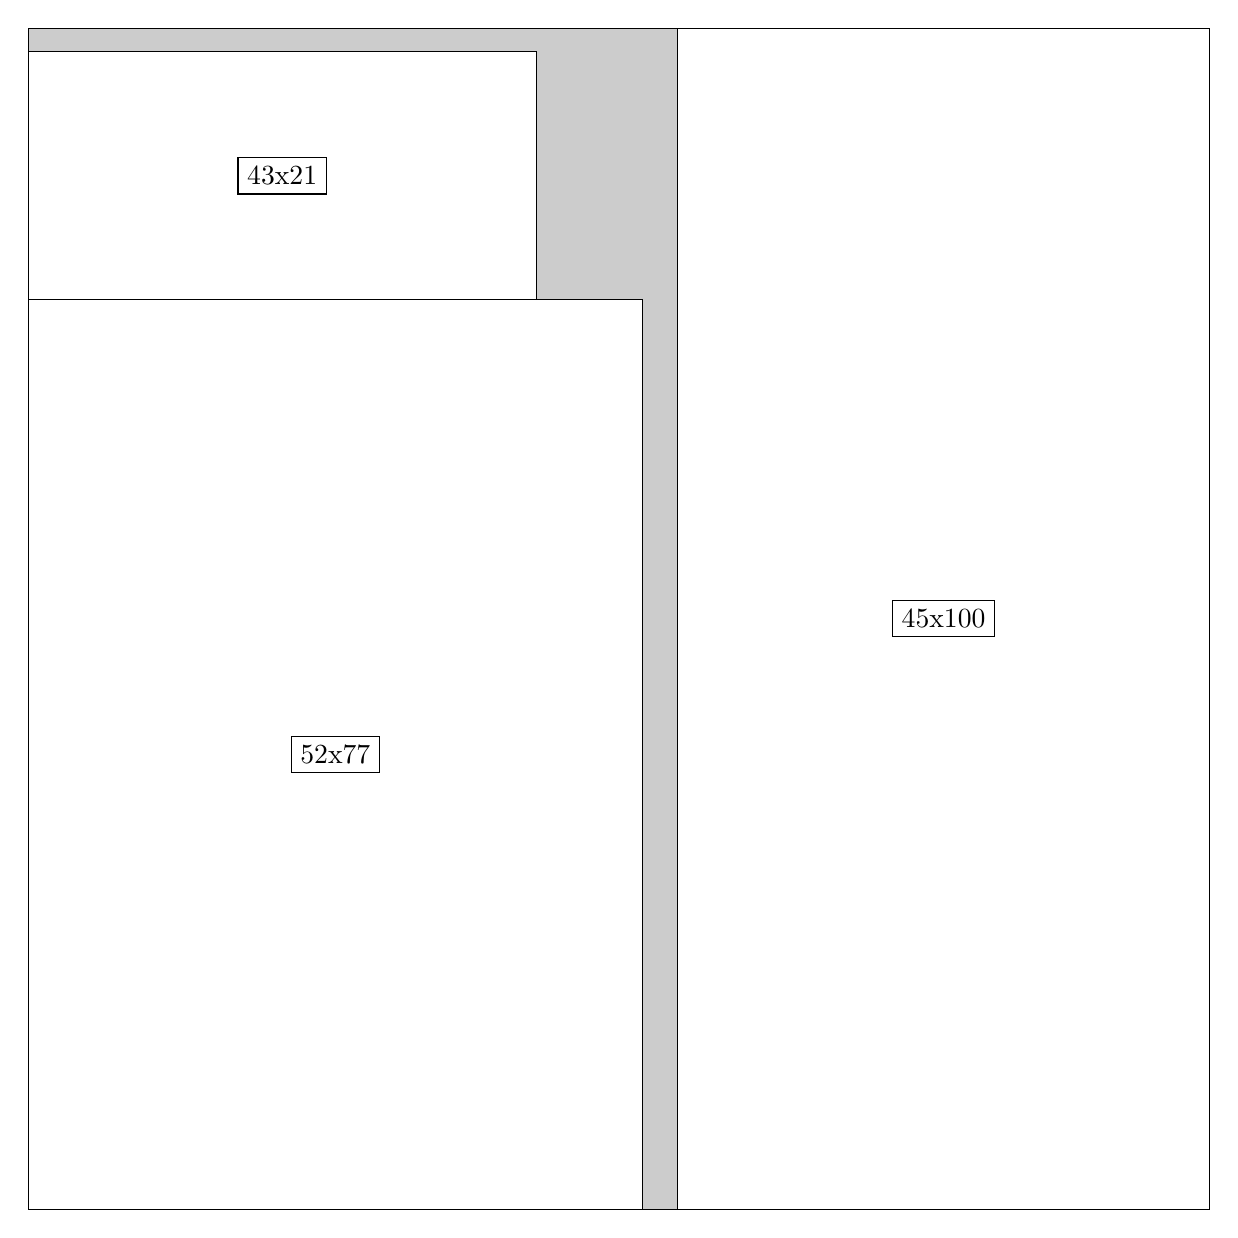
\begin{tikzpicture}[shorten >=1pt,scale=1.0,every node/.style={scale=1.0},->]
\tikzstyle{vertex}=[circle,fill=black!25,minimum size=14pt,inner sep=0pt]
\filldraw[fill=gray!40!white, draw=black] (0,0) rectangle (15.0,15.0);
\foreach \name/\x/\y/\w/\h in {45x100/8.25/0.0/6.75/15.0,52x77/0.0/0.0/7.8/11.549999999999999,43x21/0.0/11.549999999999999/6.45/3.15}
\filldraw[fill=white!40!white, draw=black] (\x,\y) rectangle node[draw] (\name) {\name} ++(\w,\h);
\end{tikzpicture}


w =45 , h =100 , x =55 , y =0 , v =4500
\par
w =52 , h =77 , x =0 , y =0 , v =4004
\par
w =43 , h =21 , x =0 , y =77 , v =903
\par
\newpage


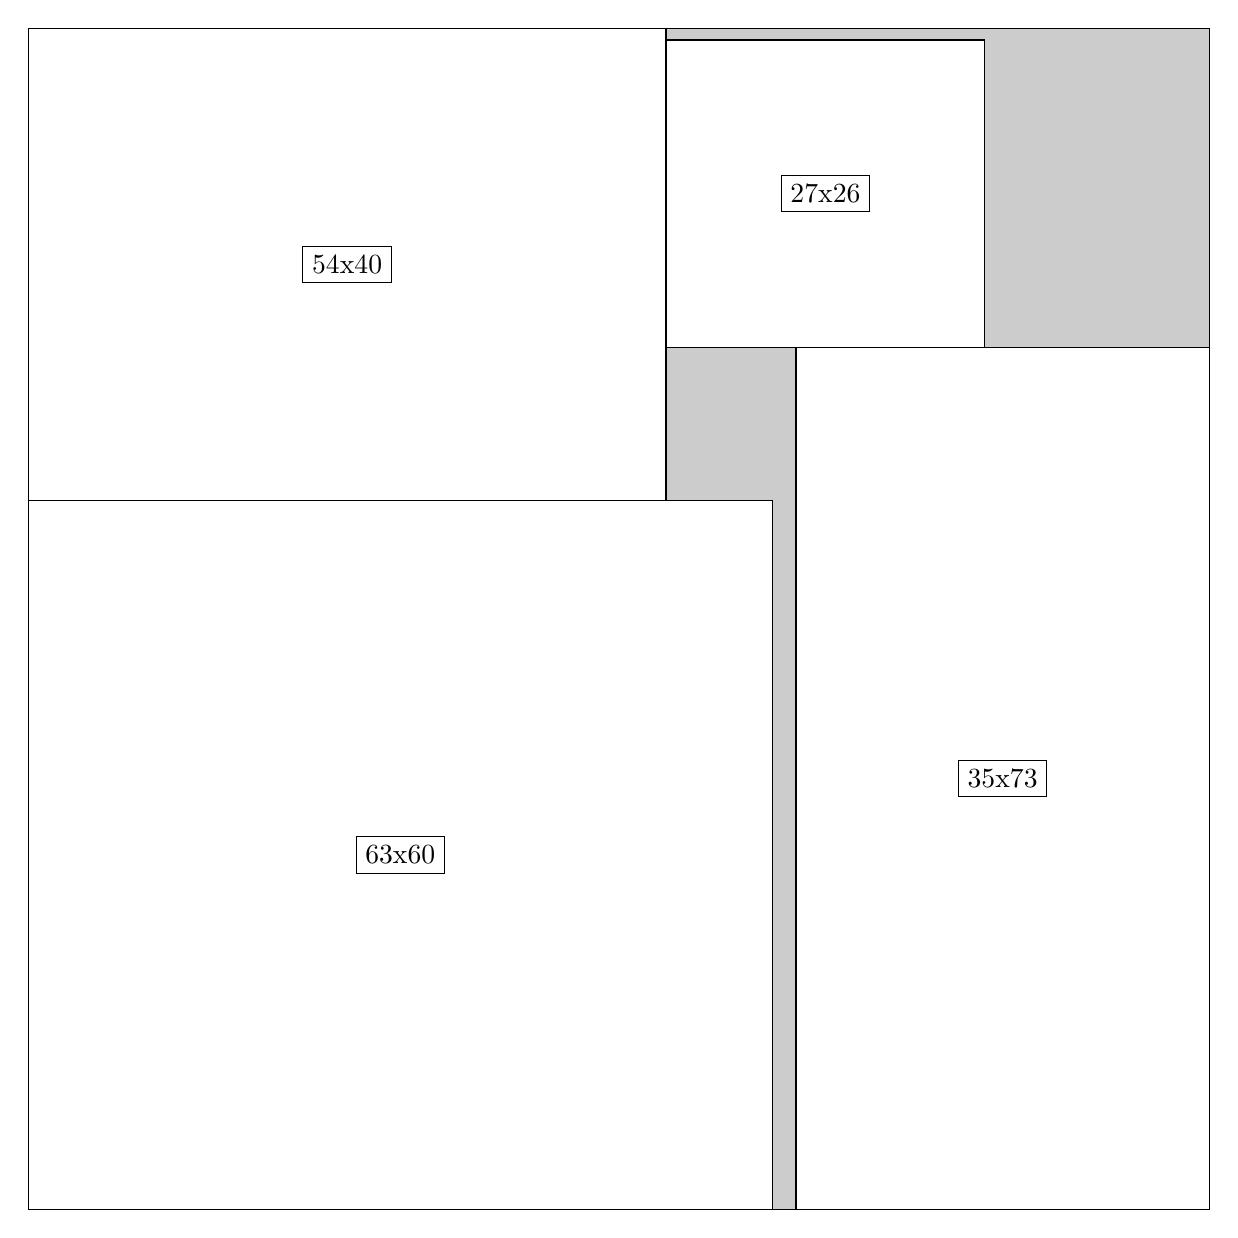
\begin{tikzpicture}[shorten >=1pt,scale=1.0,every node/.style={scale=1.0},->]
\tikzstyle{vertex}=[circle,fill=black!25,minimum size=14pt,inner sep=0pt]
\filldraw[fill=gray!40!white, draw=black] (0,0) rectangle (15.0,15.0);
\foreach \name/\x/\y/\w/\h in {63x60/0.0/0.0/9.45/9.0,35x73/9.75/0.0/5.25/10.95,54x40/0.0/9.0/8.1/6.0,27x26/8.1/10.95/4.05/3.9}
\filldraw[fill=white!40!white, draw=black] (\x,\y) rectangle node[draw] (\name) {\name} ++(\w,\h);
\end{tikzpicture}


w =63 , h =60 , x =0 , y =0 , v =3780
\par
w =35 , h =73 , x =65 , y =0 , v =2555
\par
w =54 , h =40 , x =0 , y =60 , v =2160
\par
w =27 , h =26 , x =54 , y =73 , v =702
\par
\newpage


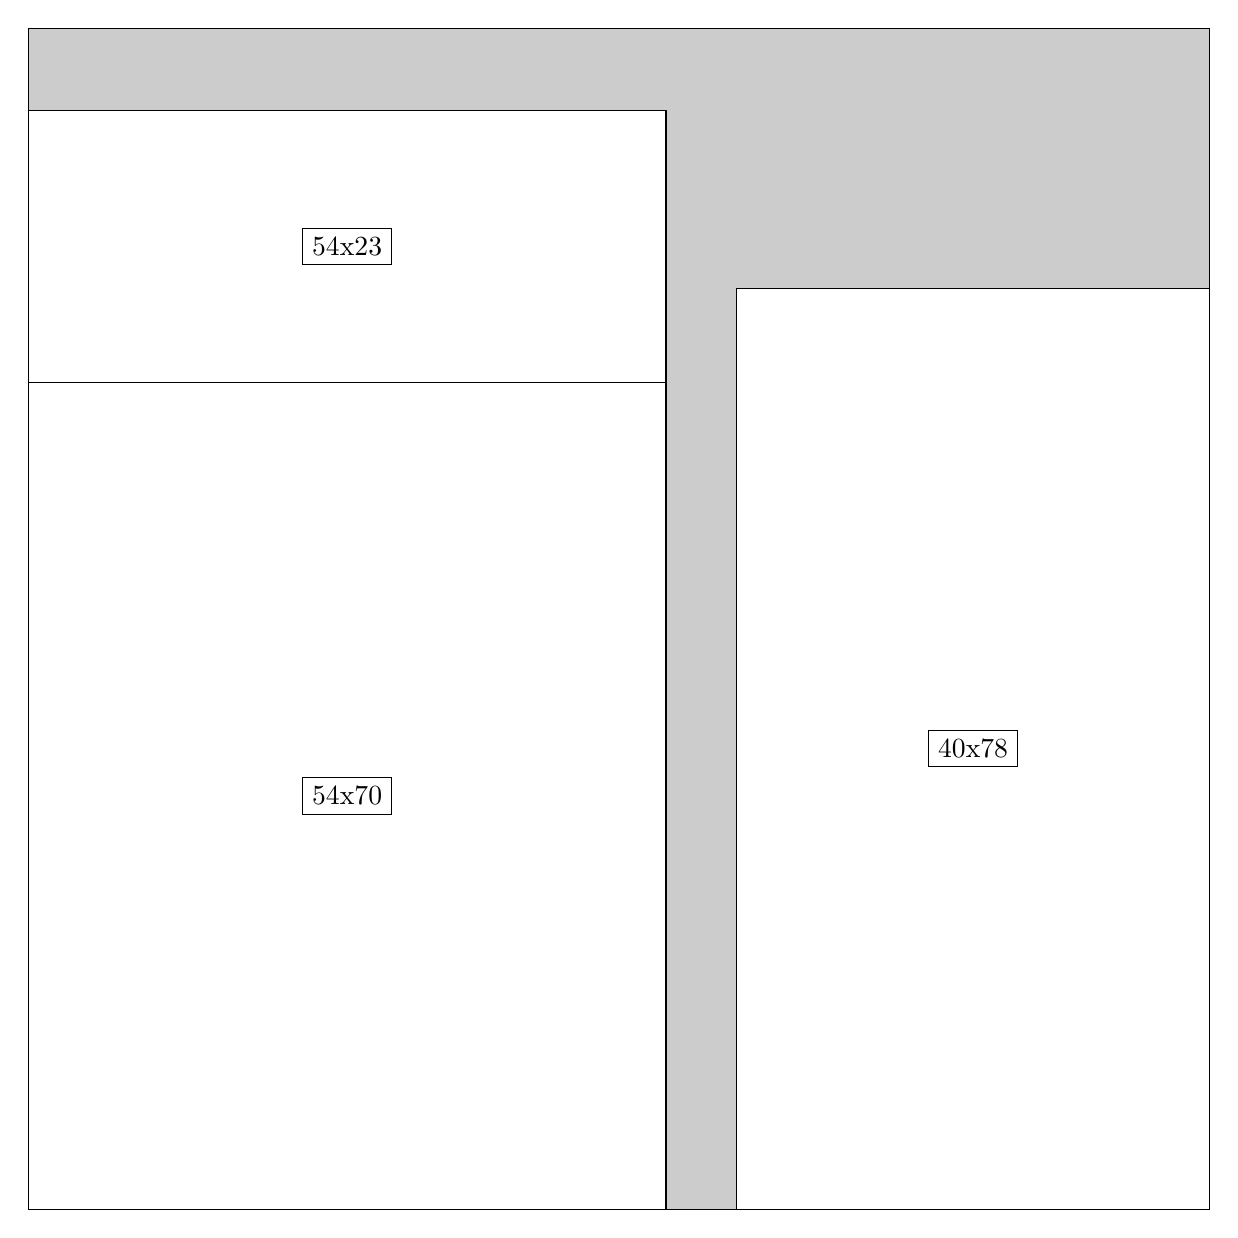
\begin{tikzpicture}[shorten >=1pt,scale=1.0,every node/.style={scale=1.0},->]
\tikzstyle{vertex}=[circle,fill=black!25,minimum size=14pt,inner sep=0pt]
\filldraw[fill=gray!40!white, draw=black] (0,0) rectangle (15.0,15.0);
\foreach \name/\x/\y/\w/\h in {54x70/0.0/0.0/8.1/10.5,40x78/9.0/0.0/6.0/11.7,54x23/0.0/10.5/8.1/3.4499999999999997}
\filldraw[fill=white!40!white, draw=black] (\x,\y) rectangle node[draw] (\name) {\name} ++(\w,\h);
\end{tikzpicture}


w =54 , h =70 , x =0 , y =0 , v =3780
\par
w =40 , h =78 , x =60 , y =0 , v =3120
\par
w =54 , h =23 , x =0 , y =70 , v =1242
\par
\newpage


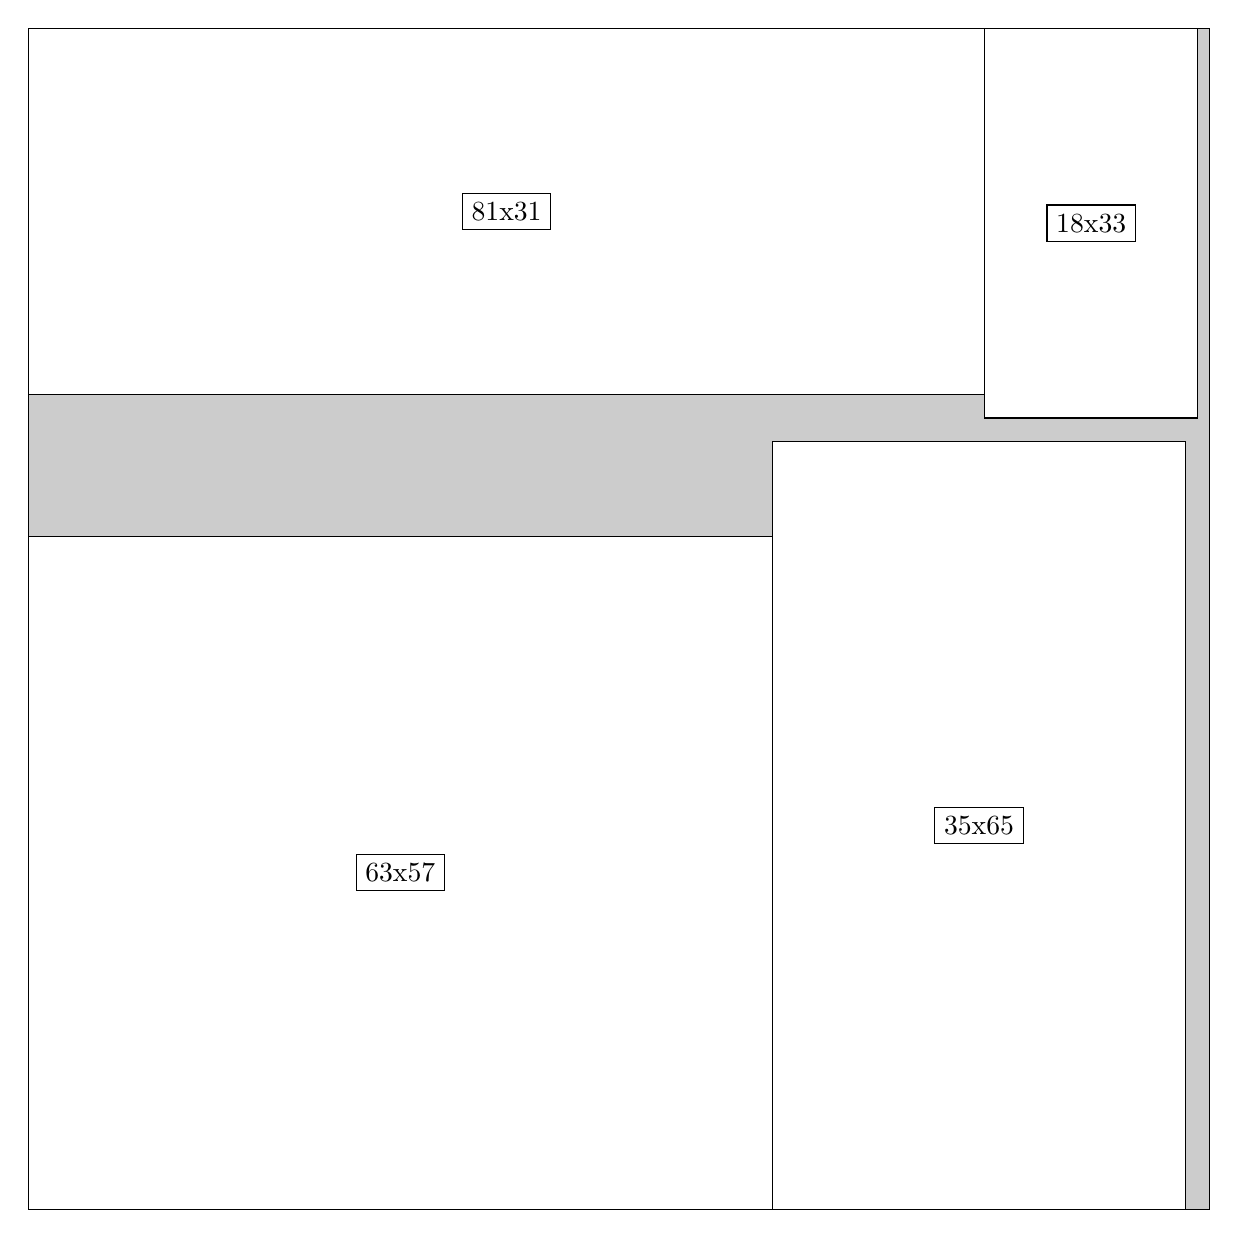
\begin{tikzpicture}[shorten >=1pt,scale=1.0,every node/.style={scale=1.0},->]
\tikzstyle{vertex}=[circle,fill=black!25,minimum size=14pt,inner sep=0pt]
\filldraw[fill=gray!40!white, draw=black] (0,0) rectangle (15.0,15.0);
\foreach \name/\x/\y/\w/\h in {63x57/0.0/0.0/9.45/8.549999999999999,81x31/0.0/10.35/12.15/4.6499999999999995,35x65/9.45/0.0/5.25/9.75,18x33/12.15/10.049999999999999/2.6999999999999997/4.95}
\filldraw[fill=white!40!white, draw=black] (\x,\y) rectangle node[draw] (\name) {\name} ++(\w,\h);
\end{tikzpicture}


w =63 , h =57 , x =0 , y =0 , v =3591
\par
w =81 , h =31 , x =0 , y =69 , v =2511
\par
w =35 , h =65 , x =63 , y =0 , v =2275
\par
w =18 , h =33 , x =81 , y =67 , v =594
\par
\newpage


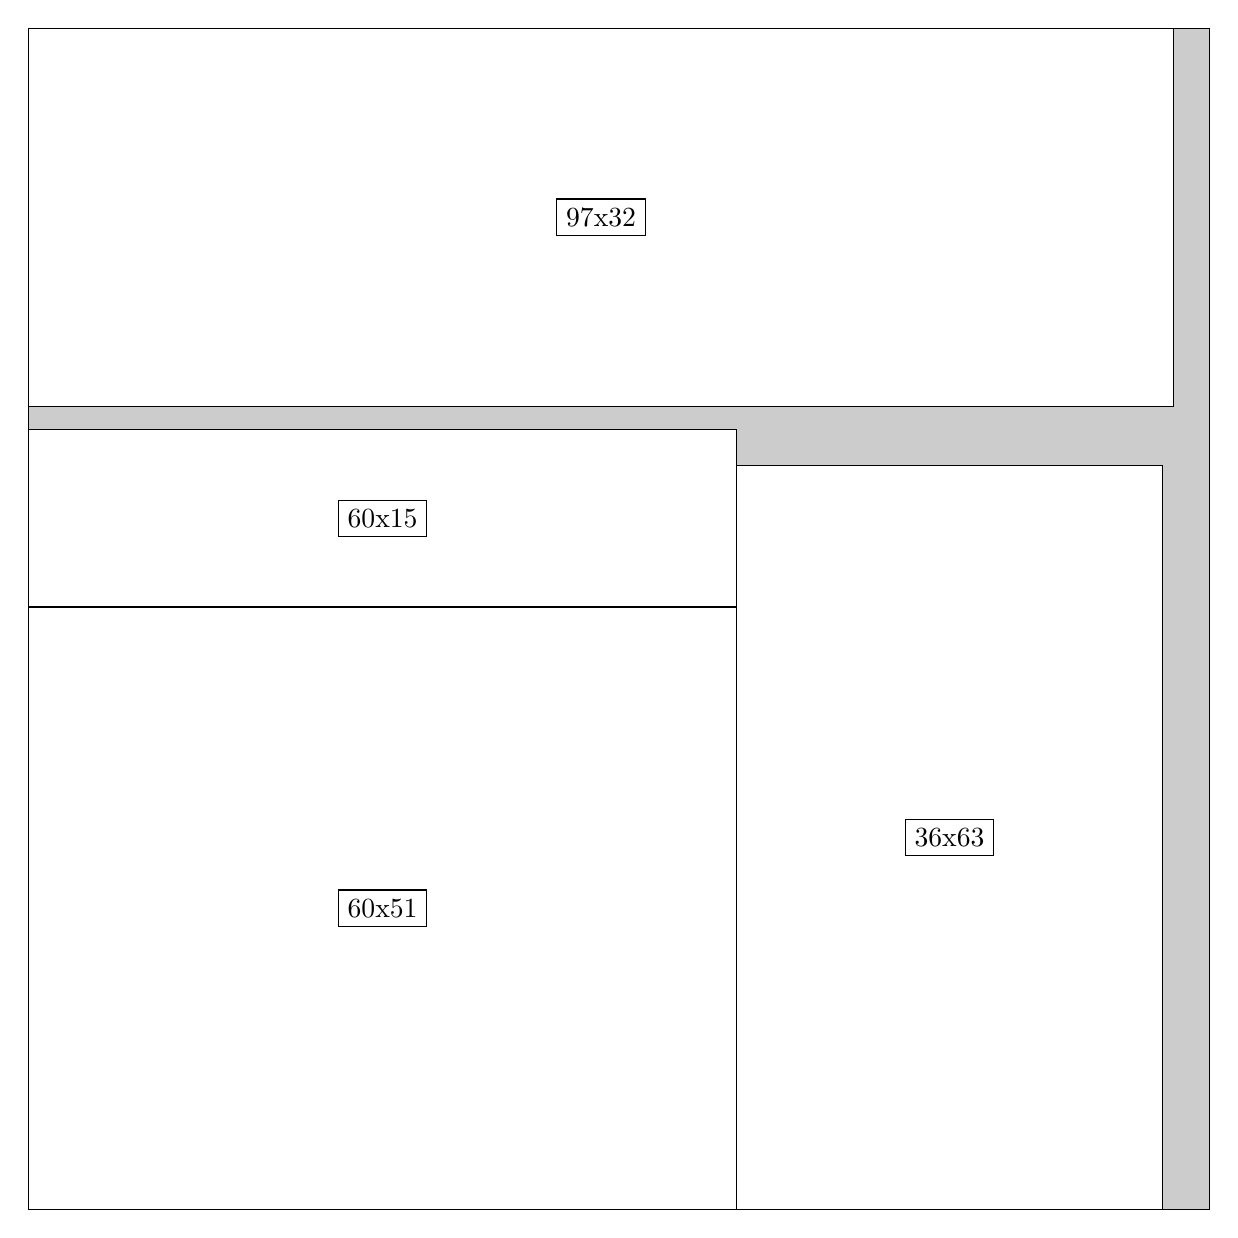
\begin{tikzpicture}[shorten >=1pt,scale=1.0,every node/.style={scale=1.0},->]
\tikzstyle{vertex}=[circle,fill=black!25,minimum size=14pt,inner sep=0pt]
\filldraw[fill=gray!40!white, draw=black] (0,0) rectangle (15.0,15.0);
\foreach \name/\x/\y/\w/\h in {97x32/0.0/10.2/14.549999999999999/4.8,60x51/0.0/0.0/9.0/7.6499999999999995,36x63/9.0/0.0/5.3999999999999995/9.45,60x15/0.0/7.6499999999999995/9.0/2.25}
\filldraw[fill=white!40!white, draw=black] (\x,\y) rectangle node[draw] (\name) {\name} ++(\w,\h);
\end{tikzpicture}


w =97 , h =32 , x =0 , y =68 , v =3104
\par
w =60 , h =51 , x =0 , y =0 , v =3060
\par
w =36 , h =63 , x =60 , y =0 , v =2268
\par
w =60 , h =15 , x =0 , y =51 , v =900
\par
\newpage


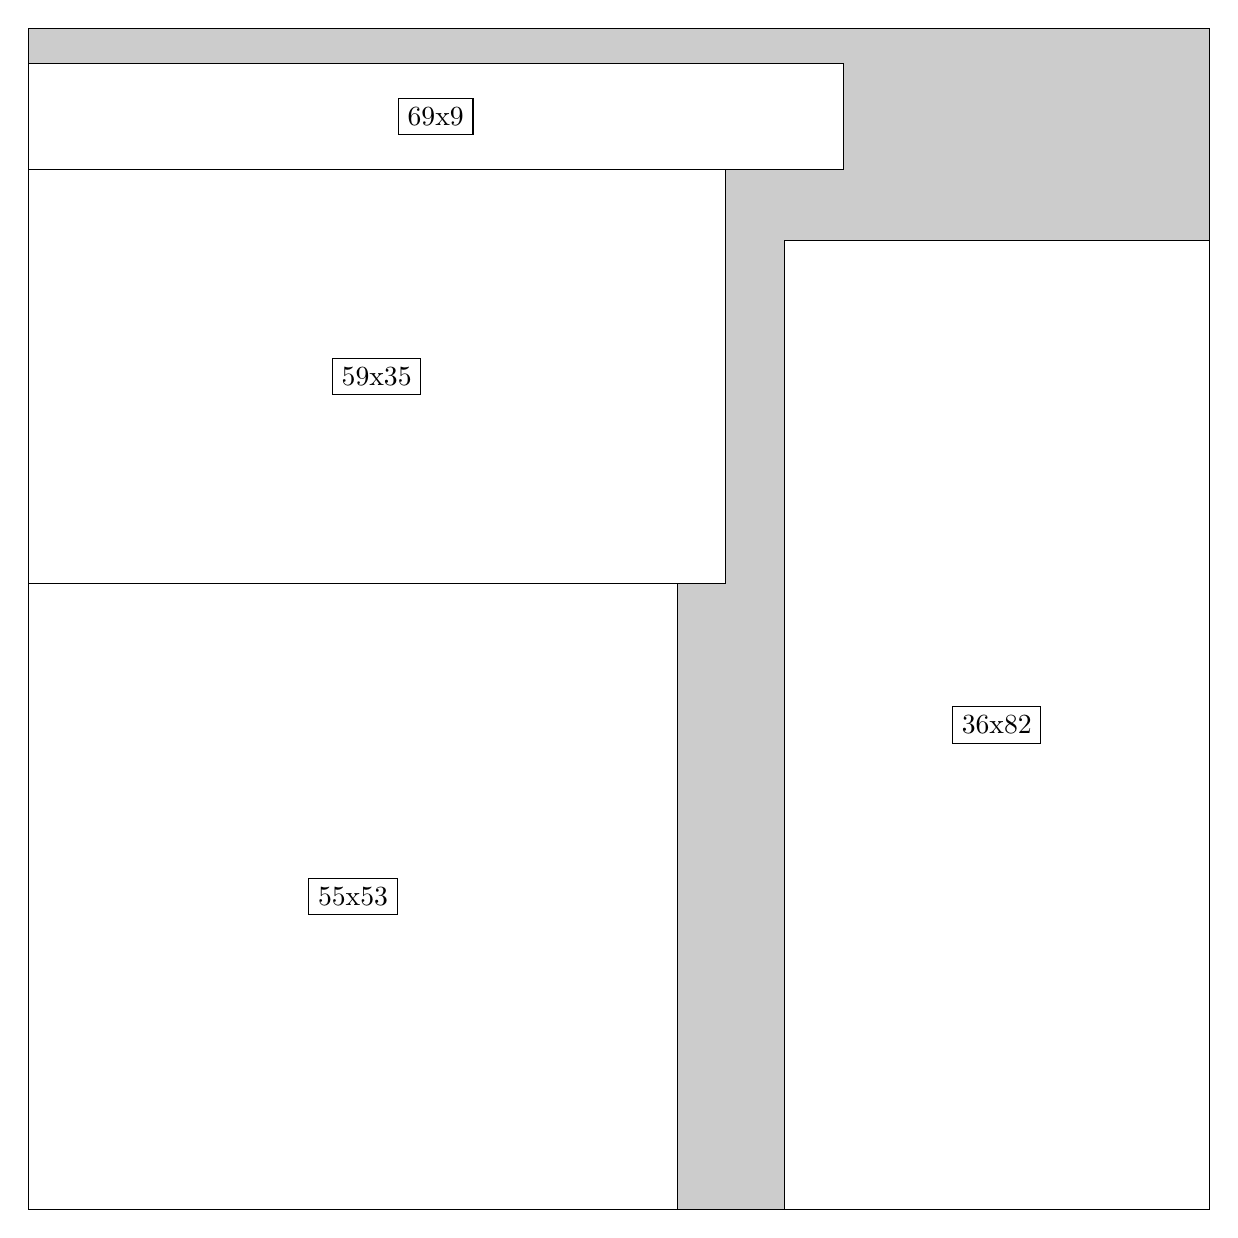
\begin{tikzpicture}[shorten >=1pt,scale=1.0,every node/.style={scale=1.0},->]
\tikzstyle{vertex}=[circle,fill=black!25,minimum size=14pt,inner sep=0pt]
\filldraw[fill=gray!40!white, draw=black] (0,0) rectangle (15.0,15.0);
\foreach \name/\x/\y/\w/\h in {36x82/9.6/0.0/5.3999999999999995/12.299999999999999,55x53/0.0/0.0/8.25/7.949999999999999,59x35/0.0/7.949999999999999/8.85/5.25,69x9/0.0/13.2/10.35/1.3499999999999999}
\filldraw[fill=white!40!white, draw=black] (\x,\y) rectangle node[draw] (\name) {\name} ++(\w,\h);
\end{tikzpicture}


w =36 , h =82 , x =64 , y =0 , v =2952
\par
w =55 , h =53 , x =0 , y =0 , v =2915
\par
w =59 , h =35 , x =0 , y =53 , v =2065
\par
w =69 , h =9 , x =0 , y =88 , v =621
\par
\newpage


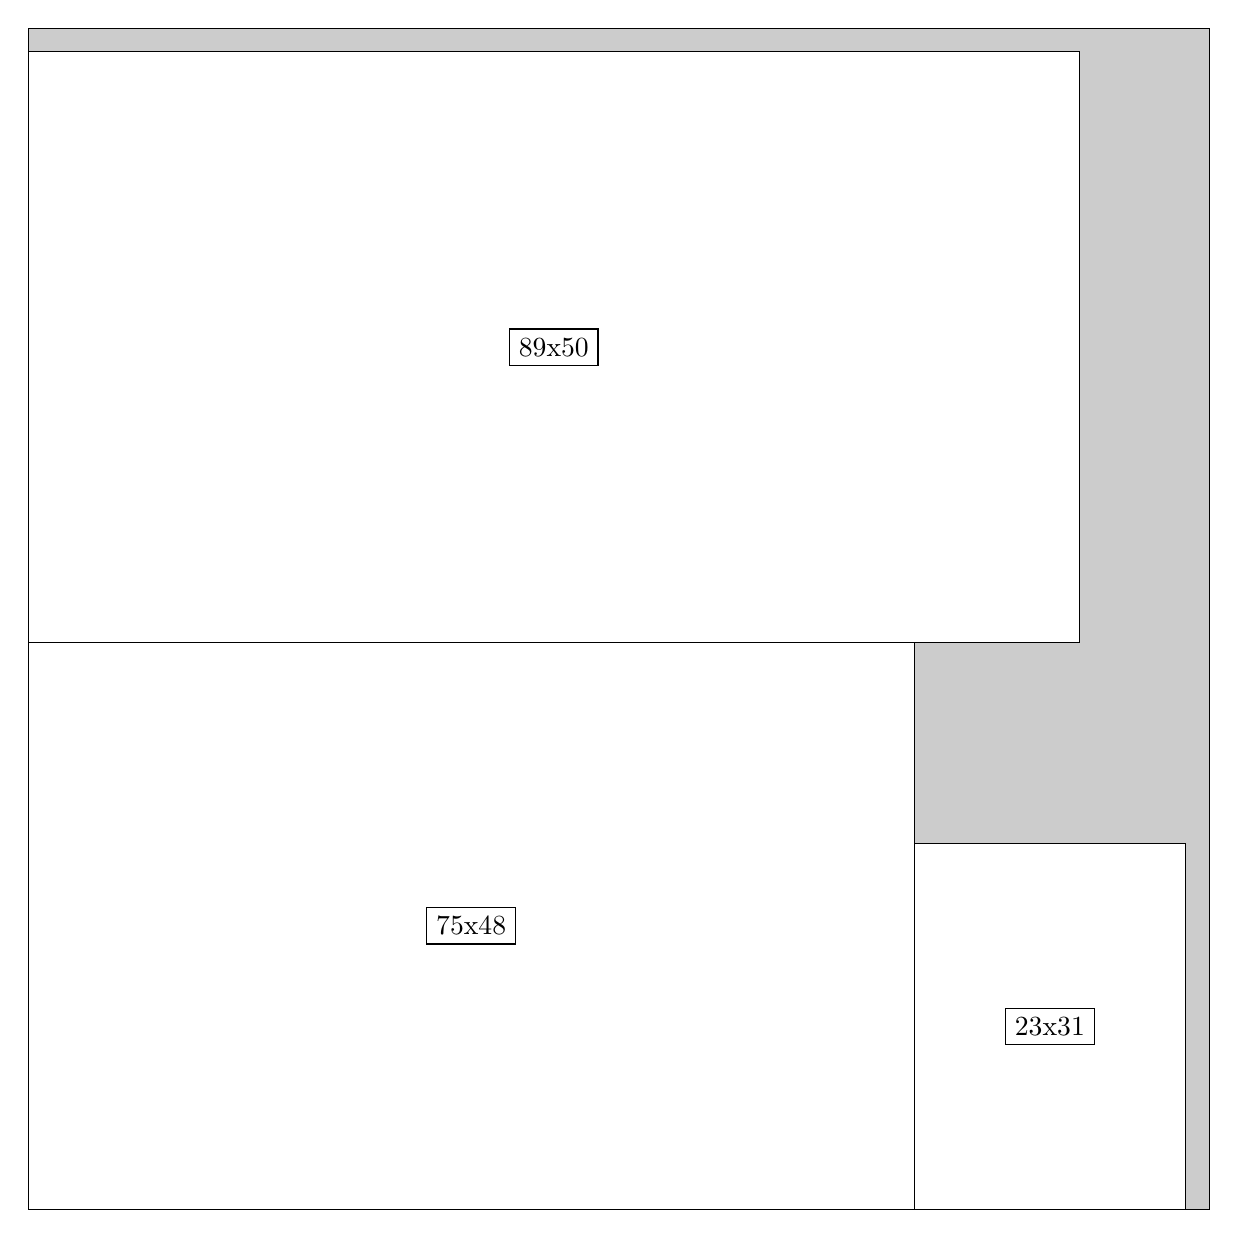
\begin{tikzpicture}[shorten >=1pt,scale=1.0,every node/.style={scale=1.0},->]
\tikzstyle{vertex}=[circle,fill=black!25,minimum size=14pt,inner sep=0pt]
\filldraw[fill=gray!40!white, draw=black] (0,0) rectangle (15.0,15.0);
\foreach \name/\x/\y/\w/\h in {89x50/0.0/7.199999999999999/13.35/7.5,75x48/0.0/0.0/11.25/7.199999999999999,23x31/11.25/0.0/3.4499999999999997/4.6499999999999995}
\filldraw[fill=white!40!white, draw=black] (\x,\y) rectangle node[draw] (\name) {\name} ++(\w,\h);
\end{tikzpicture}


w =89 , h =50 , x =0 , y =48 , v =4450
\par
w =75 , h =48 , x =0 , y =0 , v =3600
\par
w =23 , h =31 , x =75 , y =0 , v =713
\par
\newpage


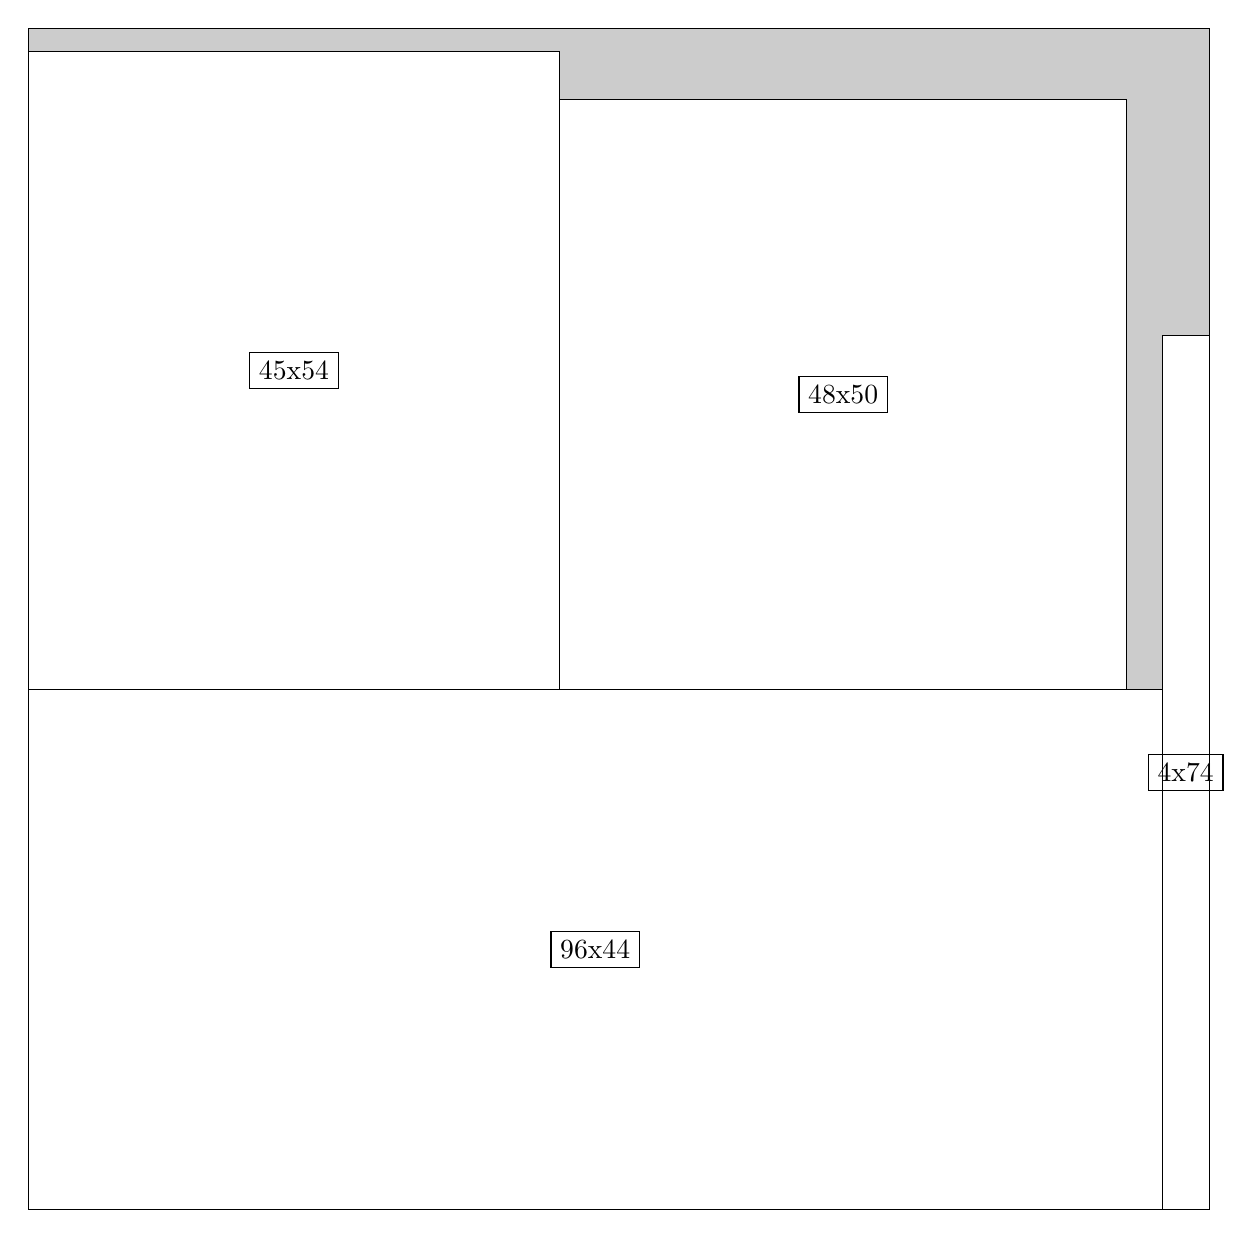
\begin{tikzpicture}[shorten >=1pt,scale=1.0,every node/.style={scale=1.0},->]
\tikzstyle{vertex}=[circle,fill=black!25,minimum size=14pt,inner sep=0pt]
\filldraw[fill=gray!40!white, draw=black] (0,0) rectangle (15.0,15.0);
\foreach \name/\x/\y/\w/\h in {96x44/0.0/0.0/14.399999999999999/6.6,45x54/0.0/6.6/6.75/8.1,48x50/6.75/6.6/7.199999999999999/7.5,4x74/14.399999999999999/0.0/0.6/11.1}
\filldraw[fill=white!40!white, draw=black] (\x,\y) rectangle node[draw] (\name) {\name} ++(\w,\h);
\end{tikzpicture}


w =96 , h =44 , x =0 , y =0 , v =4224
\par
w =45 , h =54 , x =0 , y =44 , v =2430
\par
w =48 , h =50 , x =45 , y =44 , v =2400
\par
w =4 , h =74 , x =96 , y =0 , v =296
\par
\newpage


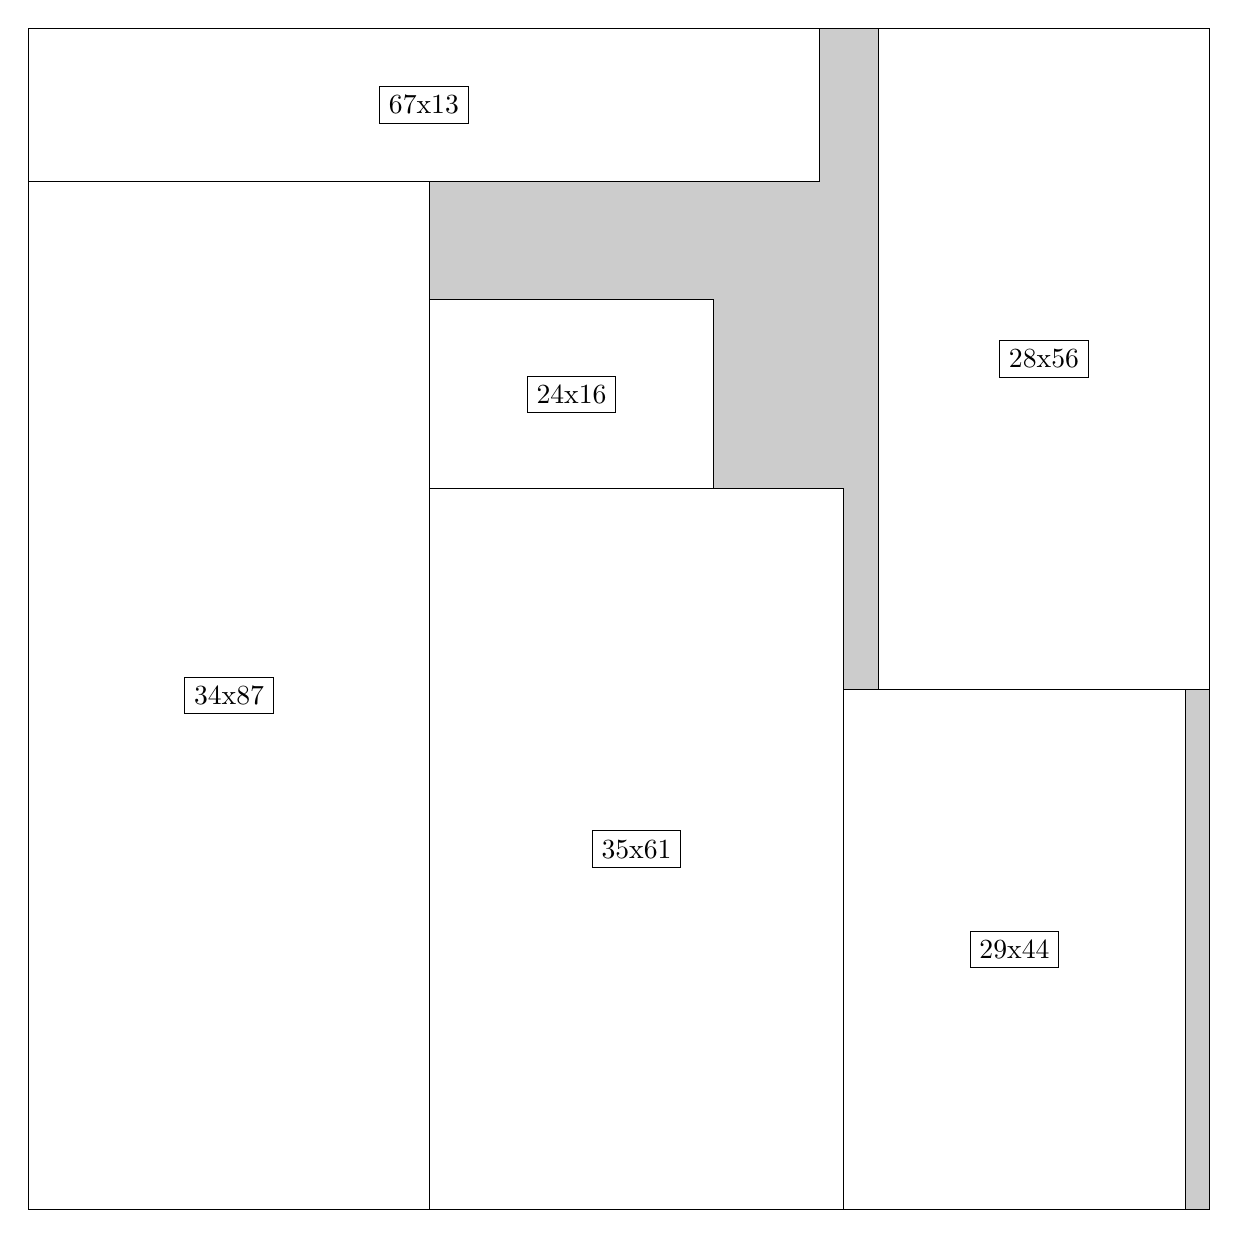
\begin{tikzpicture}[shorten >=1pt,scale=1.0,every node/.style={scale=1.0},->]
\tikzstyle{vertex}=[circle,fill=black!25,minimum size=14pt,inner sep=0pt]
\filldraw[fill=gray!40!white, draw=black] (0,0) rectangle (15.0,15.0);
\foreach \name/\x/\y/\w/\h in {34x87/0.0/0.0/5.1/13.049999999999999,35x61/5.1/0.0/5.25/9.15,28x56/10.799999999999999/6.6/4.2/8.4,29x44/10.35/0.0/4.35/6.6,67x13/0.0/13.049999999999999/10.049999999999999/1.95,24x16/5.1/9.15/3.5999999999999996/2.4}
\filldraw[fill=white!40!white, draw=black] (\x,\y) rectangle node[draw] (\name) {\name} ++(\w,\h);
\end{tikzpicture}


w =34 , h =87 , x =0 , y =0 , v =2958
\par
w =35 , h =61 , x =34 , y =0 , v =2135
\par
w =28 , h =56 , x =72 , y =44 , v =1568
\par
w =29 , h =44 , x =69 , y =0 , v =1276
\par
w =67 , h =13 , x =0 , y =87 , v =871
\par
w =24 , h =16 , x =34 , y =61 , v =384
\par
\newpage


\end{document}